%%%%%%%%%%%%%%%%%%%%%%%%%%%%%%%%%%%%%%%%%%%%%%%%%%%%%%%%%%%%%%%%%%%%%
% LaTeXTemplate: Project Titlepage Modified (v 0.1) by rcx
%
% Original Source: http://www.howtotex.com
% Date: February 2014
% 
% This is a title page template which be used for articles & reports.
% 
% This is the modified version of the original Latex template from
% aforementioned website.
% 
%%%%%%%%%%%%%%%%%%%%%%%%%%%%%%%%%%%%%%%%%%%%%%%%%%%%%%%%%%%%%%%%%%%%%%t

\documentclass[12pt]{report}
\usepackage[a4paper]{geometry}
\usepackage[myheadings]{fullpage}
\usepackage{fancyhdr}
\usepackage{lastpage}
\usepackage{subcaption}
\usepackage[colorlinks=true,linkcolor=blue]{hyperref}%


\usepackage{graphicx, wrapfig, subcaption, setspace, booktabs}
\usepackage[T1]{fontenc}
\usepackage[font=small, labelfont=bf]{caption}
%\usepackage{fourier}
\usepackage[protrusion=true, expansion=true]{microtype}
\usepackage[english]{babel}
\usepackage{sectsty}
\usepackage{url, lipsum}

\usepackage{graphicx}
\usepackage{booktabs}
\usepackage{float}
\usepackage{amsmath}
\usepackage{amssymb}
\usepackage{url}
\usepackage{hyperref}
\usepackage{booktabs}
\usepackage{longtable}
\usepackage{url}
\usepackage{hyperref}
\usepackage{mathabx}
\usepackage{natbib}
\newcommand*\mean[1]{\overline{#1}}


\newcommand{\HRule}[1]{\rule{\linewidth}{#1}}
\onehalfspacing
\setcounter{tocdepth}{5}
\setcounter{secnumdepth}{5}

%-------------------------------------------------------------------------------
% HEADER & FOOTER
%-------------------------------------------------------------------------------
\pagestyle{fancy}
\fancyhf{}
\setlength\headheight{15pt}
\fancyhead[R]{Oana Vesa}
\fancyhead[L]{Merging Elliptical Galaxies}

\fancyfoot[R]{Page \thepage\ of \pageref{LastPage}}
%-------------------------------------------------------------------------------
% TITLE PAGE
%-------------------------------------------------------------------------------

\begin{document}

\title{ \normalsize \textsc{}
		\\ [2.0cm]
		\HRule{0.5pt} \\
		\LARGE \textbf{\uppercase{Merging Elliptical Galaxies}}
		\HRule{2pt} \\ [0.5cm]
		\normalsize \today \vspace*{5\baselineskip}}

\date{}

\author{ ASTR 506  \\
		Oana Vesa}

\maketitle
\tableofcontents
\newpage

%-------------------------------------------------------------------------------
% Section title formatting
\sectionfont{\scshape}
%-------------------------------------------------------------------------------

%-------------------------------------------------------------------------------
% BODY
%-------------------------------------------------------------------------------

\section*{Abstract}
\addcontentsline{toc}{section}{Abstract}

An investigation into the dynamics of two merging elliptical galaxies of $20,000$ equally massed particles was conducted. Using equations of motion and a constant time-step leap-frog integration scheme (KDK, or Kick Drift Kick), two merger models were created. The first merger configuration had the two elliptical galaxies offset by an x-shift of $50$ and a y-shift of $20$. The second merger model had the two elliptical galaxies offset by an x-shift of $150$ and a y-shift of $20$. Both models were given an equal but opposite velocity kick in the x-, y-, and z-direction of $\pm 0.2$, $\pm 0.1$, and $\pm 0.02$, respectively. The effects on their velocities, energies, number of particles lost, density, and angular momentum following these mergers were explored.

\newpage

\section*{Introduction}
\addcontentsline{toc}{section}{Introduction}

Studying the merger of galaxies is important for better understanding galaxy formation, which is a major area of research. Around the beginning of the Big Bang, the universe was pretty dense. At this point, galaxy mergers should have been frequent and should have been an integral role in galaxy evolution~\citep{mergers}. Galaxies are generally split into three broad categories: blue cloud, red sequence, and green valley. Galaxies within the blue cloud are typically galaxies undergoing star formation, such as spiral galaxies. Galaxies under the category of red sequence are galaxies that are dead and red, such as elliptical galaxies. The green valley is an in-between transition from the blue cloud to the red sequence. For instance, the Milky Way Galaxy is considered a green valley galaxy. The main question for astronomers is, what causes these galaxies to transition between these categories?

Mergers are split into two categories: wet and dry. Wet mergers tend to occur between gas-rich galaxies and should trigger star formation~\citep{2008ApJ}. Thus, the galaxy could transition from the red sequence to the blue cloud. However, dry mergers occur between gas-poor galaxies and can quench star formation, producing more red galaxies~\citep{2008ApJ}. Thus, the galaxy could transition from the blue cloud to the red sequence. Both these scenarios are important in furthering our understanding of galaxy evolution. However, it is not always easy to observe galaxy mergers. Mergers last billions of years, and it becomes difficult to constrain the merger~\citep{2008MNRAS}. 

Thus, n-body simulations are extremely useful in understanding these phenomenon. N-body simulations utilize the same equations of motions used in this report but also can account for the hydrodynamics of the system and cosmology, which this report does not. By doing this, galaxy mergers can be modeled to give astronomers more insight into the process.


\section*{Methods and Tests}
\addcontentsline{toc}{section}{Methods and Tests}

\begin{table}[H] \centering
\begin{tabular}{@{}ccc@{}} 
\toprule
\multicolumn{3}{c}{\textbf{Merger Models}} \\ \midrule
\multicolumn{1}{c|}{} & \textbf{Merger 1} & \textbf{Merger 2} \\ \cmidrule(l){2-3} 
\multicolumn{1}{c|}{\textbf{x}} & 50 & 150 \\
\multicolumn{1}{c|}{\textbf{y}} & 20 & 20 \\
\multicolumn{1}{c|}{\textbf{$\epsilon$}} & 0.001 & 0.001 \\
\multicolumn{1}{c|}{\textbf{Time}} & 300 & 500 \\
\multicolumn{1}{c|}{\textbf{dt}} & 0.1 & 0.1 \\ \bottomrule
\end{tabular}
\caption{Summary of Mergers}
\label{tab:Models}
\end{table}

The dynamics of two merging elliptical galaxies of $20,000$ equally massed particles was investigated in Fortran. Two different models were conducted--the summarized view of each configuration can be seen in Table~\ref{tab:Models} above. The initial elliptical galaxy contained $20,000$ particles, had an initial starting radius of $0.5$ to avoid the particles from flying away immediately, and an initial gaussian distribution to create the spherical shape. The elliptical galaxy was let to evolve for $8,720$ orbits. The elliptical galaxy formed can be seen in Figure~\ref{fig:cloudstructure}. By copying this galaxy, another one can be created that is equal to test different merging configurations.

 Each merging galaxy simulation was given some equal but opposite velocity kick to put the galaxies into orbit around one another. They were also given a different x and y position (the z coordinate was left alone). The acceleration loop that governs the equations of motions was parallelized using OpenMP. Parallelization is an important tool for simulations with thousands of particles. It utilizes the cores of computing clusters so that multiple processes can be conducted simultaneously. This helps in not using a lot of CPU.

The main equation that governs the formation of the elliptical galaxies in these simulations is the equation of motion,
\begin{equation} \label{eqn:equationofmotion}
    \vec{g} = -G \sum_{j=1, i \neq j}^{N} \frac{m_j \left( \vec{r_i} - \vec{r_j} \right)}{| \vec{r_i} - \vec{r_j} |^3},
\end{equation}
where $g$ is the gravitational acceleration, $G$ is the gravitational constant, $m_{j}$ is the mass of the $j^{th}$ particle, $N$ is the number of particles, and $\vec{r}$ is the position of the corresponding particles. This equation of motion is split up into three components for the x-, y-, and z-direction. Other important equations to take into account are the potential energy
\begin{equation}\label{eqn:potential_energy}
W = - \frac{1}{2} \sum_{i,j}^{N}
\frac{Gm_im_j}{| \vec{r_i} - \vec{r_j} |}    
\end{equation}
and the kinetic energy
\begin{equation}\label{eqn:kineticenergy}
K = - \frac{1}{2} \sum_{i}^N m_i \left( \vec{v_i} \right)^2.
\end{equation}

To avoid the particles having very large accelerations at small distances, a method called the Plummer softening, or force softening, was used. This insures that the simulation is stable. The Plummer softening is introduced by adding $\epsilon^2$ to the denominator of Equations~\ref{eqn:equationofmotion} and \ref{eqn:potential_energy} like so
\begin{equation} \label{eqn:plummersofteningeqnofmoiton}
\vec{g} = -G \sum_{j=1, i \neq j}^{N} \frac{m_j \left( \vec{r_i} - \vec{r_j} \right)}{(| \vec{r_i} - \vec{r_j} | + \epsilon^2 )^{3/2}}
\end{equation}
and 
\begin{equation}\label{eqn:potenitalsoftening}
    W = - \frac{1}{2} \sum_{i,j}^{N}
\frac{Gm_im_j}{| \vec{r_i} - \vec{r_j} | + \epsilon^2} .
\end{equation}


\begin{figure}[H]
\centering 
    \begin{subfigure}[b]{.475\textwidth}
        \centering
        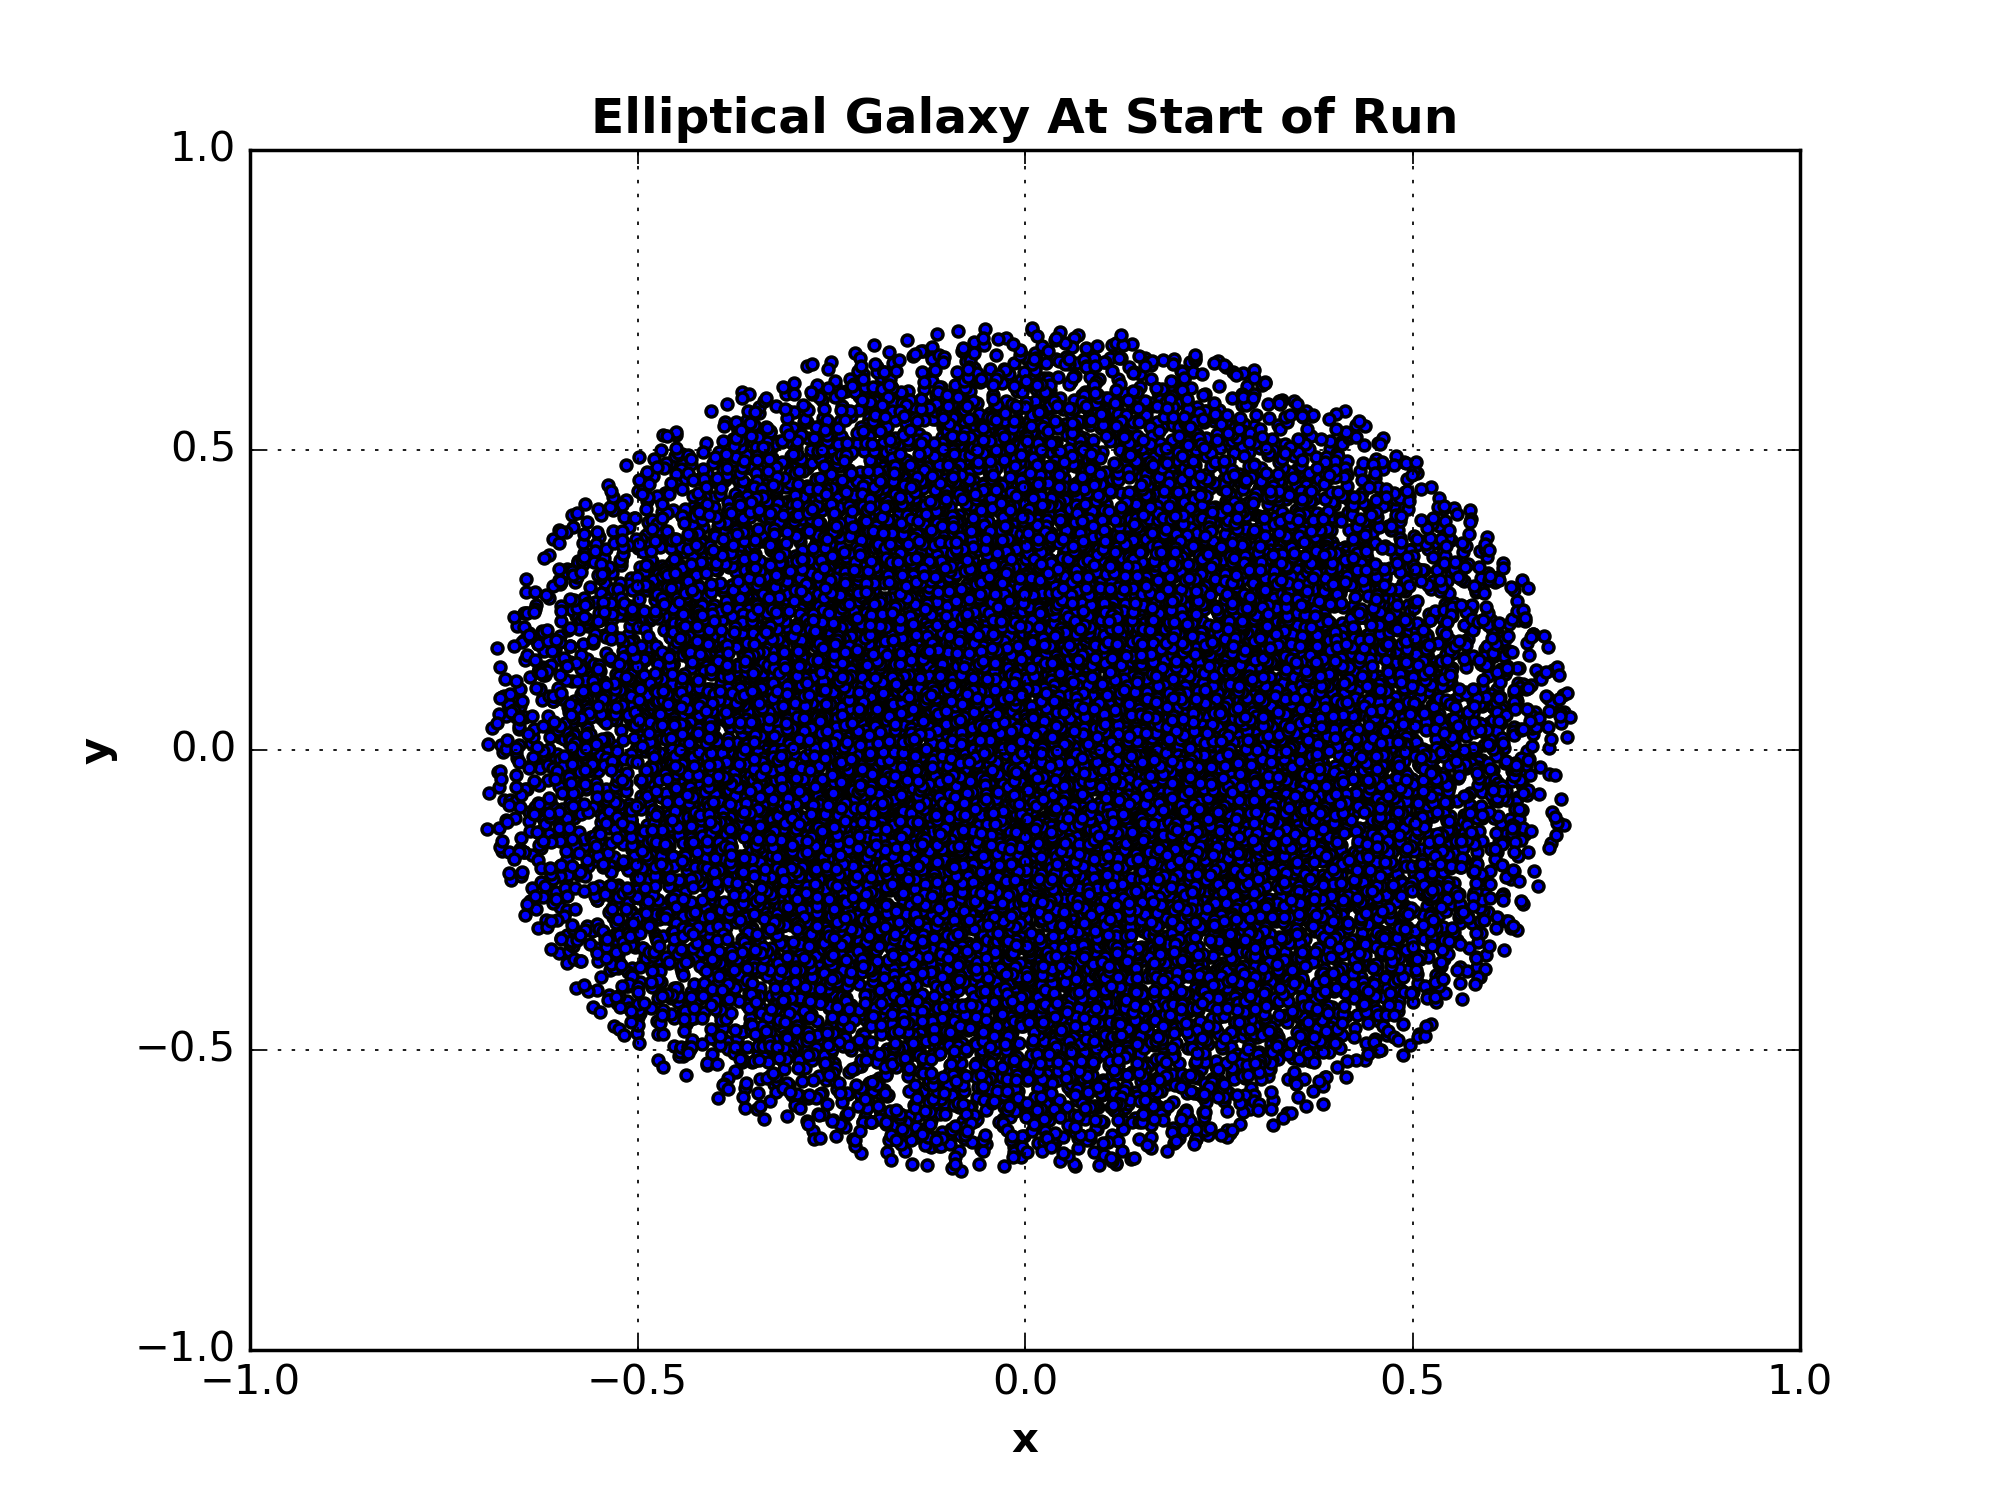
\includegraphics[width=\linewidth]{intiial_structure_of_cloud.png}
        \caption[]%
        {{\small This is the initial structure of the galaxy.}}
        \label{fig:initialstruct}
    \end{subfigure} %'
    \hfill
    \begin{subfigure}[b]{.475\textwidth}
        \centering
        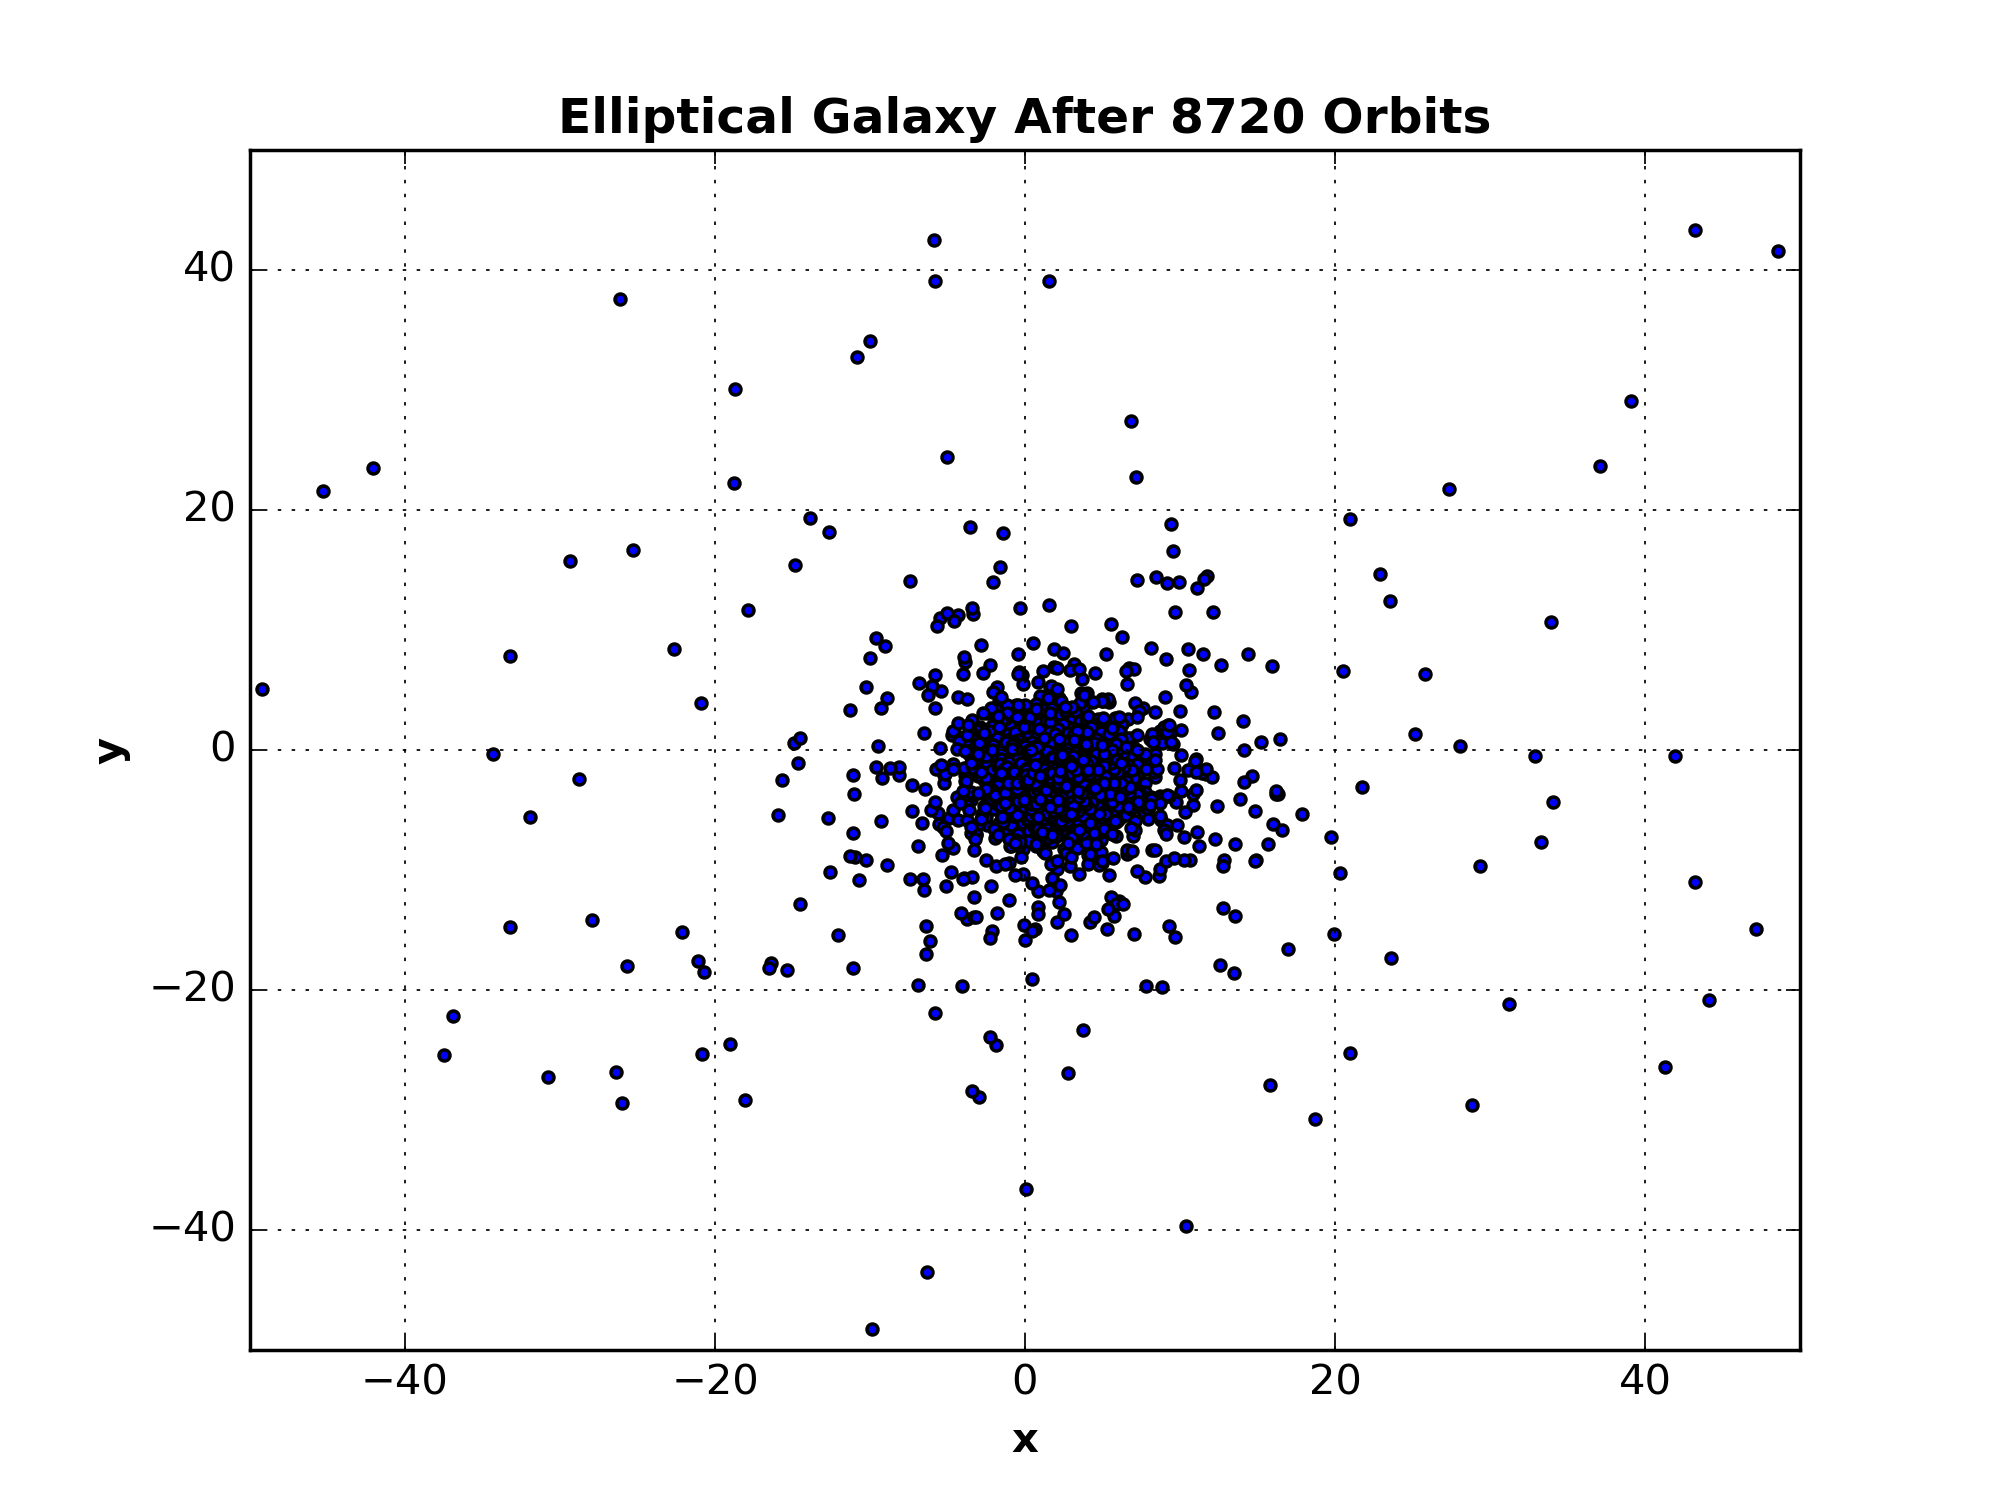
\includegraphics[width=\linewidth]{final_structure_of_cloud.png}
        \caption[]%
        {{\small This is the final structure of the galaxy.}}
        \label{fig:finalstr}
    \end{subfigure} %
    \caption[]
        {The plots above illustrate the structure of the elliptical galaxy of $20,000$ particles with a gaussian distribution after an evolution of $8,720$ dynamical orbits.} 
        \label{fig:cloudstructure}
\end{figure}


The integration scheme utilized to create the elliptical galaxy in Figure~\ref{fig:cloudstructure} was the constant time-step leap-frog (KDK or Kick Drift Kick) and direct summation to compute the accelerations. In the KDK integration scheme, the time steps are divided in half to ensure that the velocity and position coordinates meet up simultaneously. KDK works by updating the velocity coordinates (called a kick), updating the positions coordinates afterwards (called a drift), updating acceleration, and then updating velocity again. The KDK integration was used due to the fact that the orbit does not drift as much as the other integration schemes; however, some drift was present in the formation of the first initial cloud of $20,000$ particles--as can be seen in Figure~\ref{fig:finalstr}.





\section*{Analytical Estimates} \label{sec:analytical}
\addcontentsline{toc}{section}{Analytical Estimates}

The merger models allowed for the analysis of various details of the system. This report summarizes the mergers effect on the number of particles that escaped the system, the velocity, the density, and the angular momentum.

\begin{table}[H]
\begin{tabular}{@{}lcccc@{}}
\toprule
\multicolumn{5}{c}{\textbf{Particles Lost}} \\ \midrule
\multicolumn{1}{l|}{} & \multicolumn{1}{c|}{\textbf{Beginning of Merger}} & \multicolumn{1}{c|}{\textbf{During Merger}} & \multicolumn{1}{c|}{\textbf{After Merger}} & \multicolumn{1}{c|}{\textbf{Percentage Lost}} \\ \midrule
\multicolumn{1}{l|}{\textbf{Merger 1}} & $39656$ & $39633$ & $38712$ & \multicolumn{1}{c|}{$2.4\%$} \\ \midrule
\multicolumn{1}{c|}{\textbf{Merger 2}} & $39656$ & $38152$ & $35638$ & \multicolumn{1}{c|}{$10\%$} \\ \bottomrule
\end{tabular}
\caption{Number of Escaped Particles}
\label{tab:escapedparticles}
\end{table}


By defining a radius that encompasses most of the mass of the evolved elliptical galaxies during the merger, the number of particles that have escaped from the system(s) can be determined. This can be seen in Table~\ref{tab:escapedparticles} above. The calculation of the number of particles that have escaped can be determined by creating a histogram of the system, binning out to a certain diameter, and then counting all of the particles within that diameter. 

\begin{figure}[H]
    \centering
    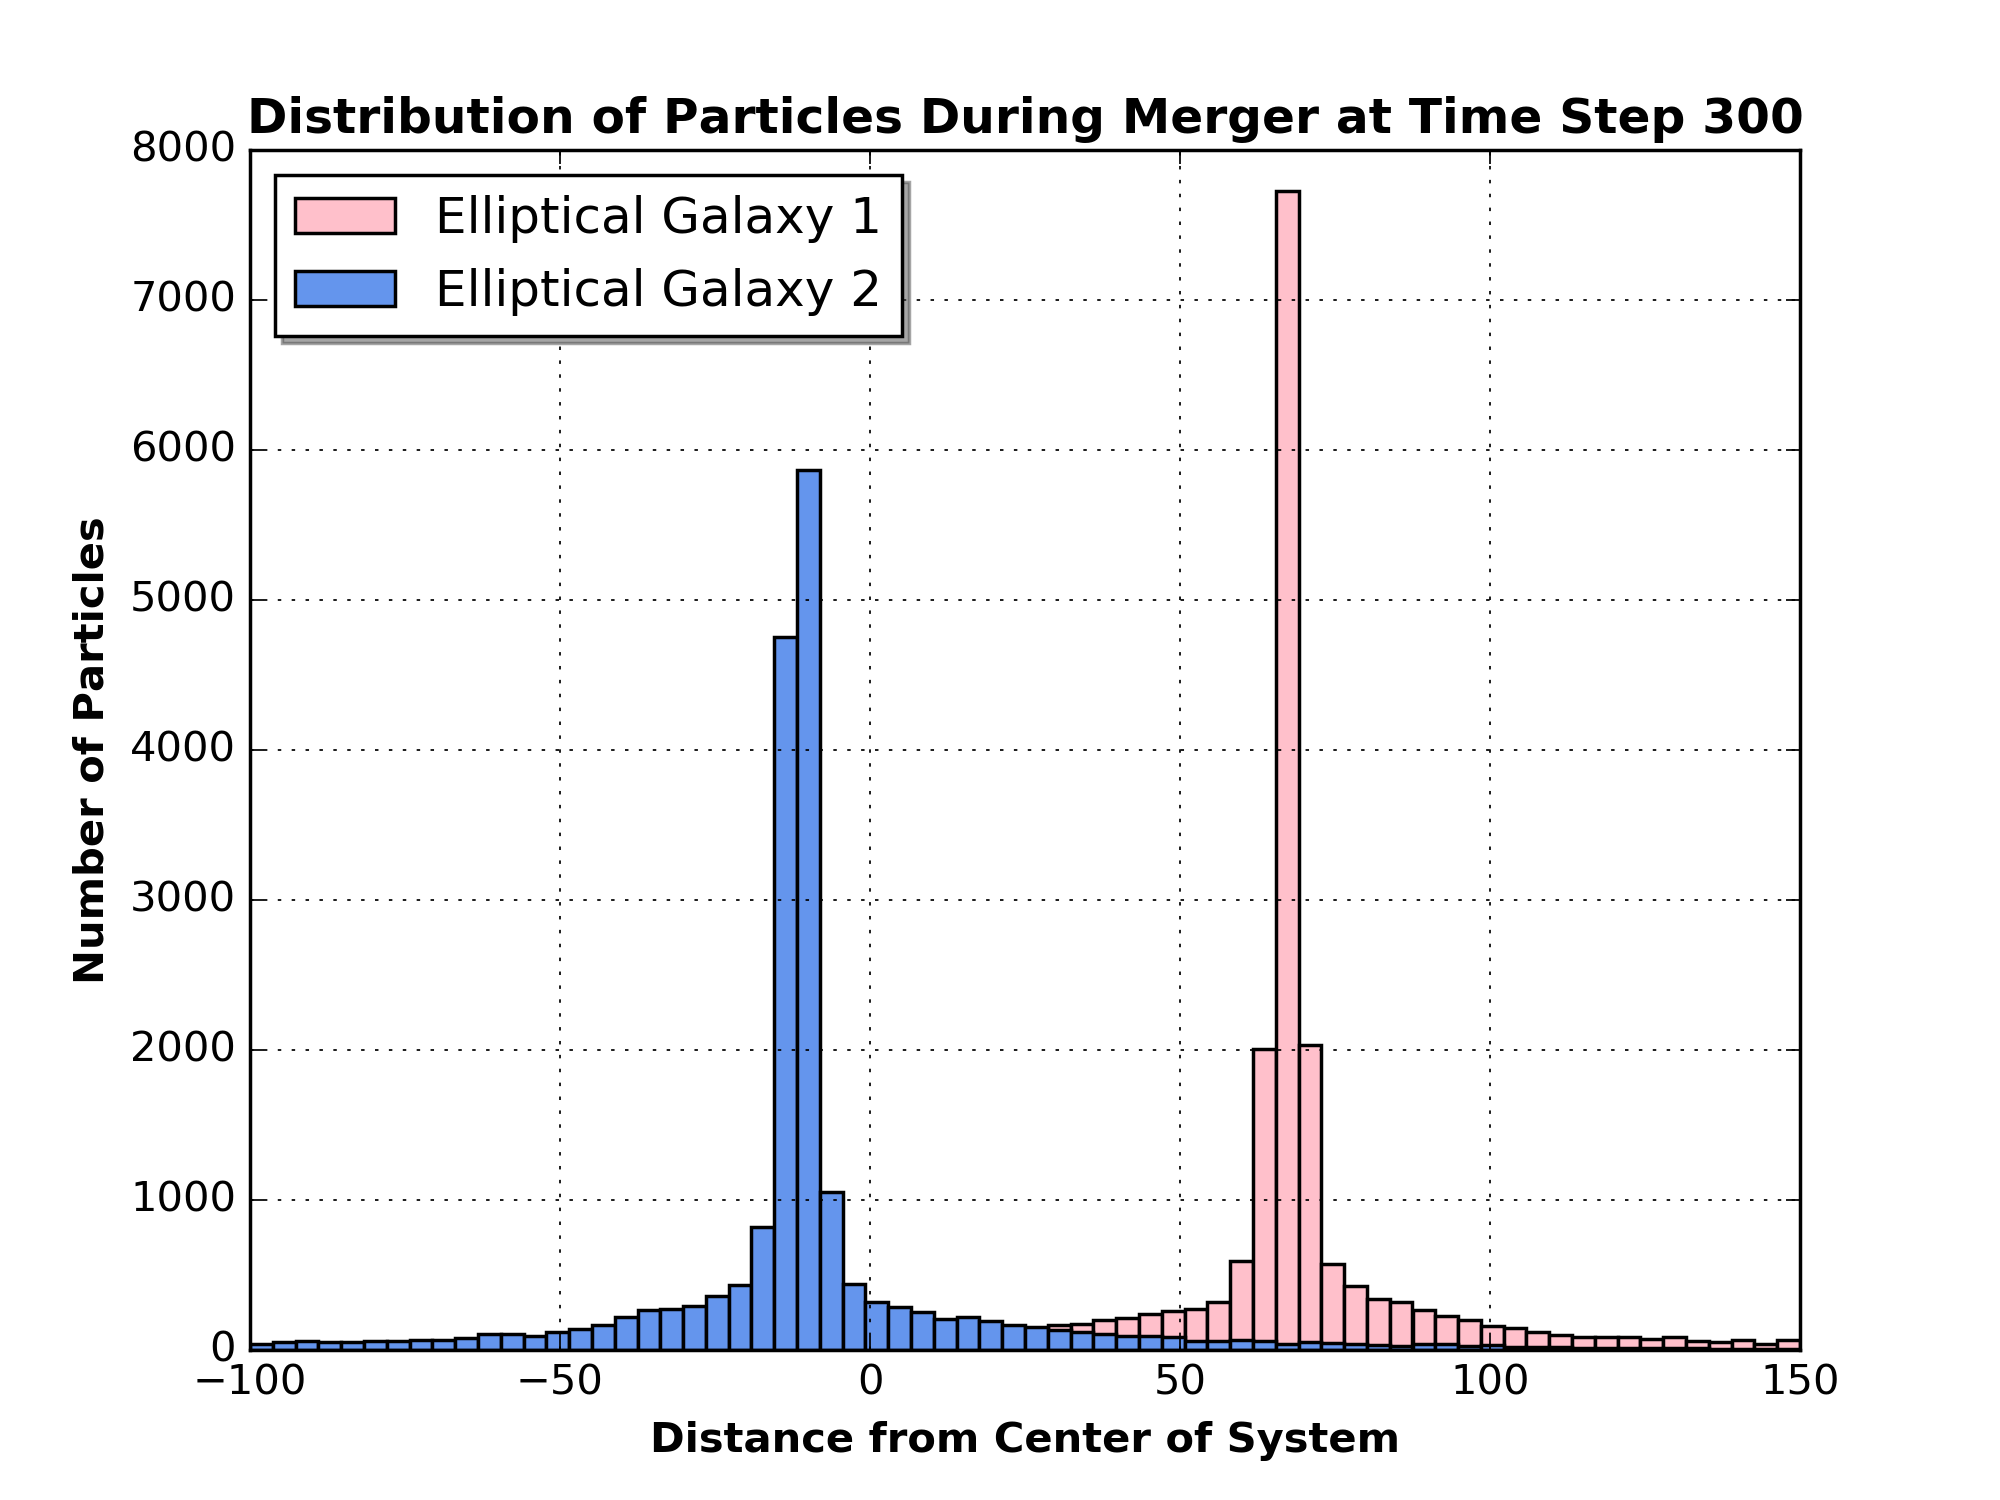
\includegraphics[scale=0.5]{histogram_final_distributionofparticlesfromcenter_aftermerger.png}
    \caption{A histogram showing the distribution of particle after the merger in the first merger model.}
    \label{fig:histdist_merger1}
\end{figure}

For instance, as seen in Figure~\ref{fig:histdist_merger1} above, by doing this, one can account for a majority of the system without worrying about the particles located further out than this predetermined diameter surrounding the merger of the two systems. By summing up all of the particles in all the bins, the number of particles that have escaped, $38,712$ particles, can be determined. This number is seen in the first row of Table~\ref{tab:escapedparticles}.




\begin{figure}[H]
\minipage{0.32\textwidth}
  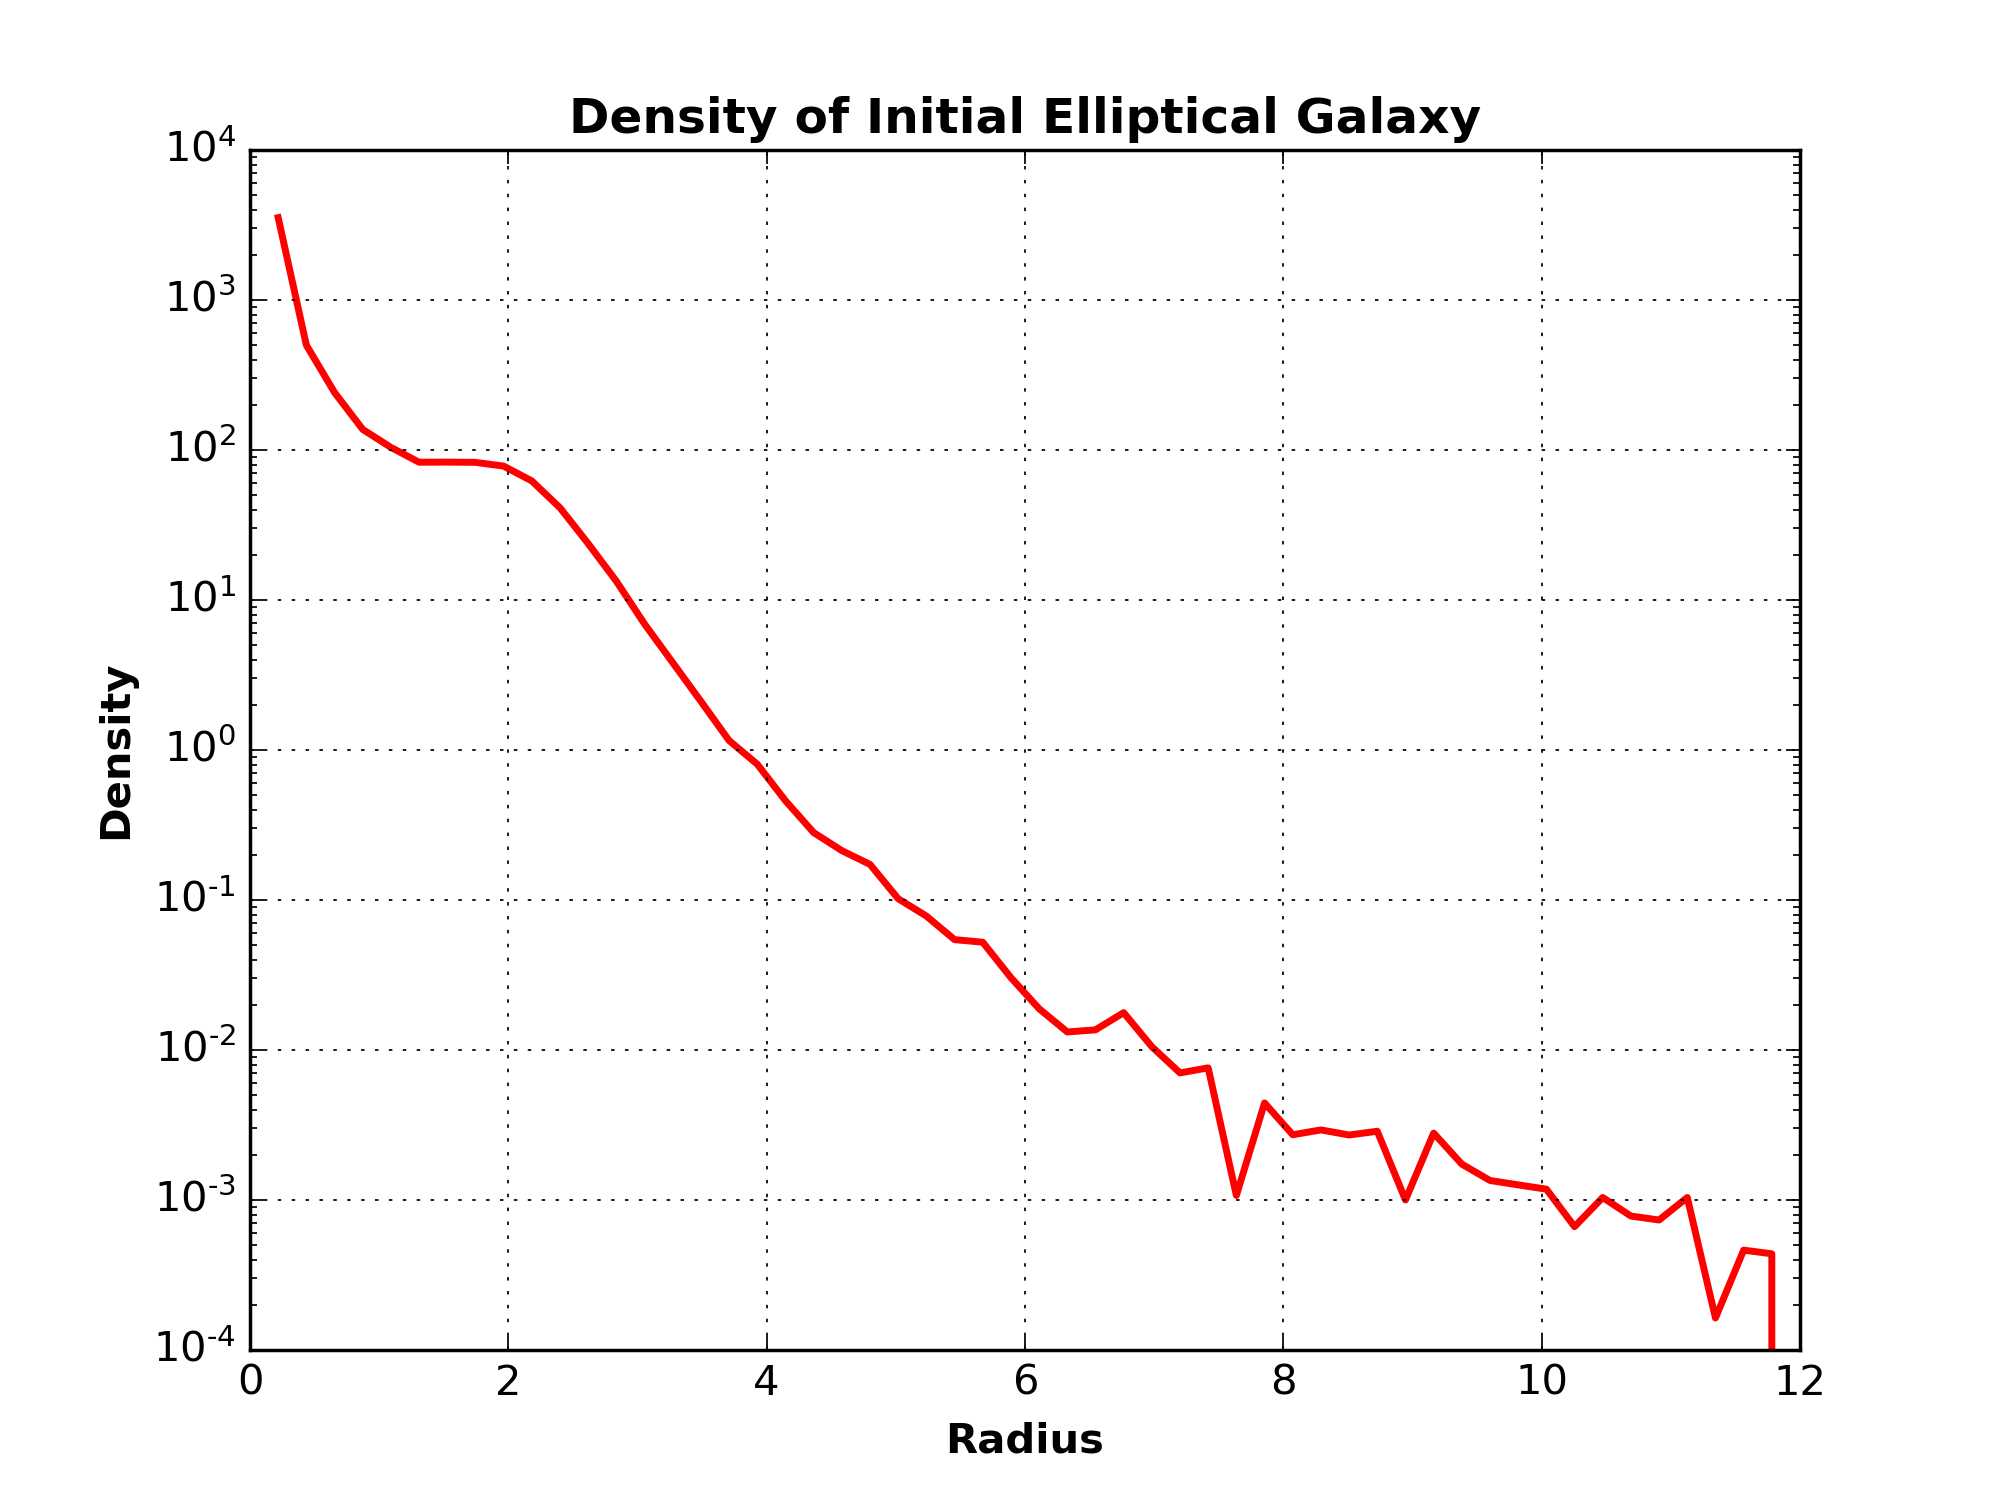
\includegraphics[width=\linewidth]{initial_density.png}
  \caption{The initial density.}
  \label{fig:density_initial}
\endminipage\hfill
\minipage{0.32\textwidth}
  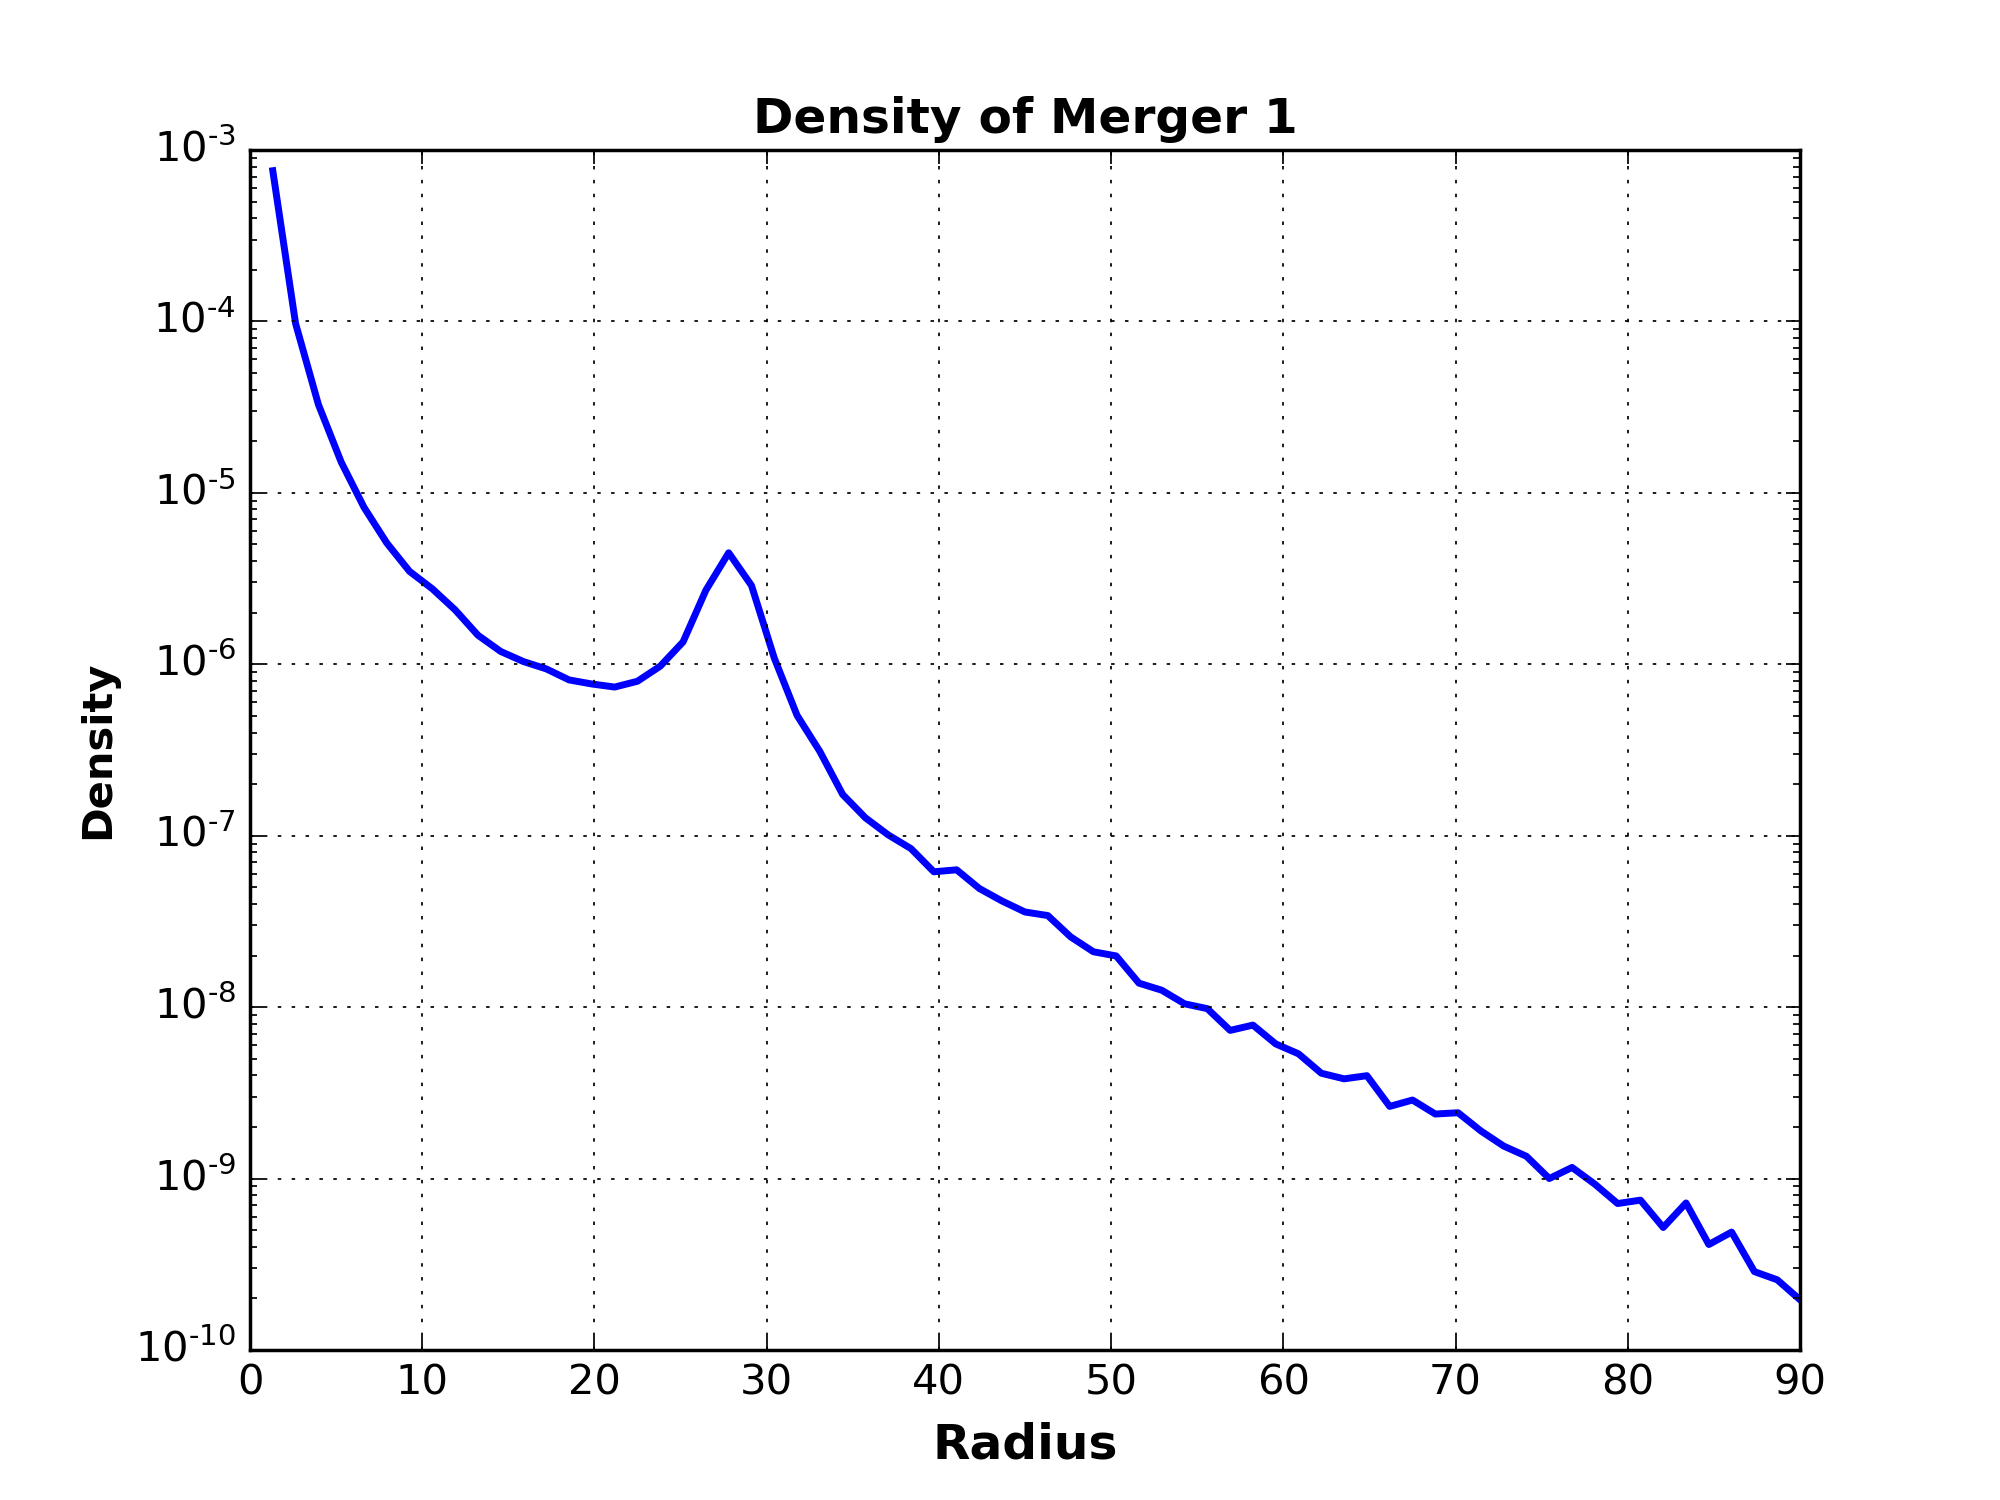
\includegraphics[width=\linewidth]{density_merger1.png}
  \caption{The density of the system after merger 1.}\label{fig:density_merger1}
\endminipage\hfill
\minipage{0.32\textwidth}
  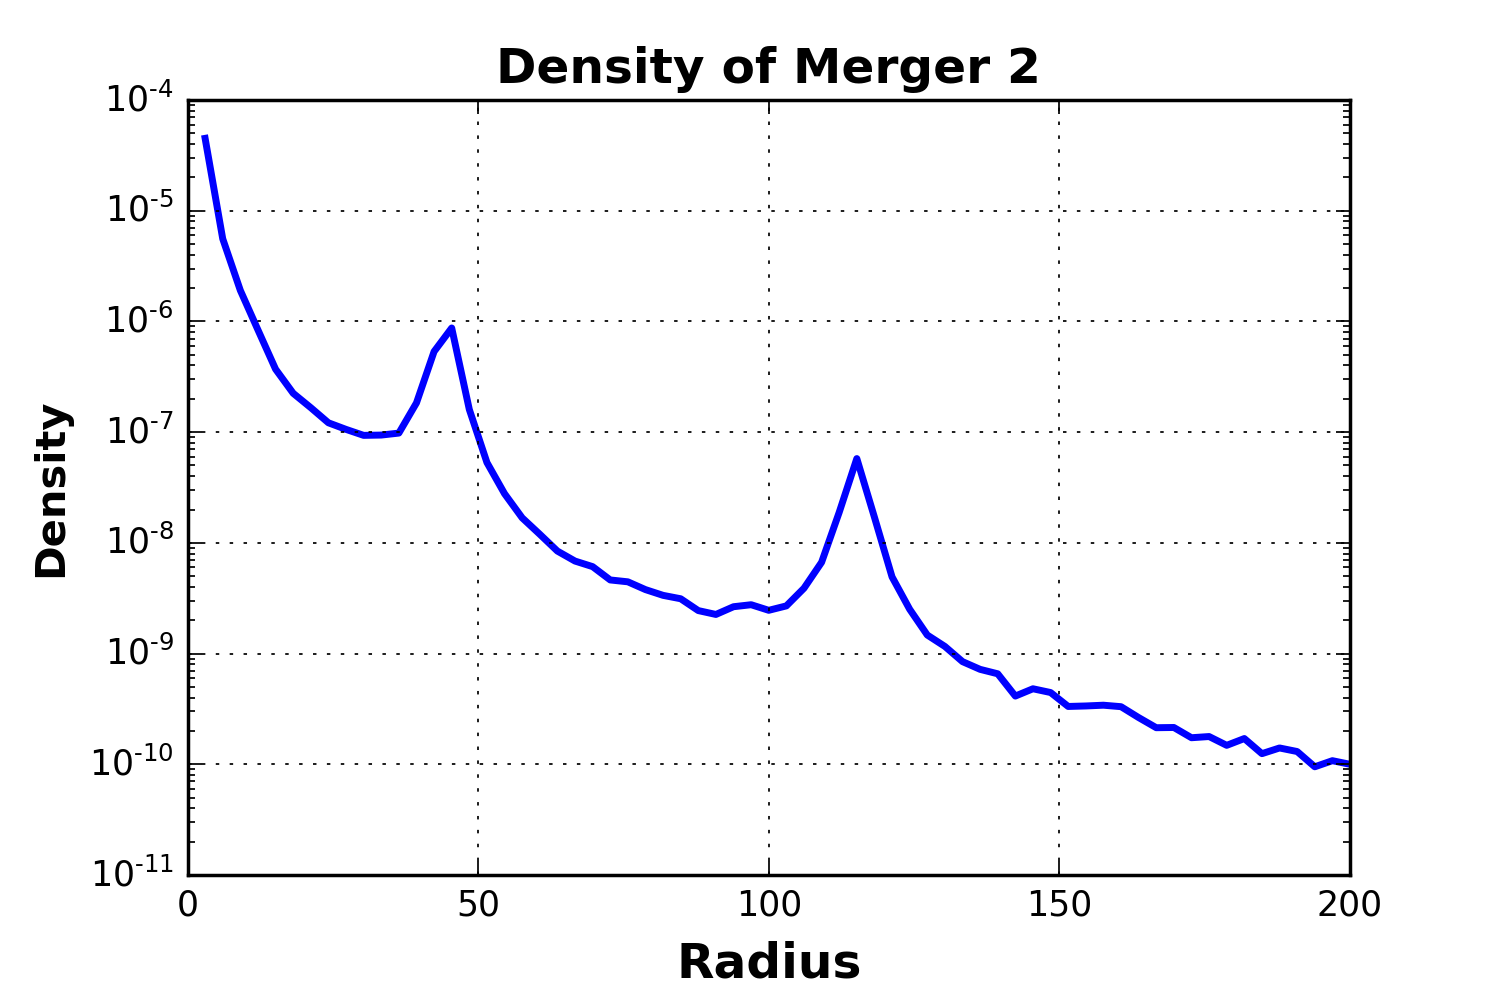
\includegraphics[width=\linewidth]{density_merger2.png}
  \caption{The density of the system after merger 2.}
  \label{fig:density_merger2}
\endminipage\hfill


\end{figure}


The density of the elliptical galaxies were determined by defining a radius around the center of the system, where most of the mass was concentrated, to some distance out that still held a substantial amount of particles. Upon determining the radius steps for this, the following equation was used to determine the density
\begin{equation}\label{eqn:density_eqn}
    \rho = \frac{M}{V},
\end{equation}
where $\rho$ is the density of the system, $M$ is the mass of the system (and since all the particles have equal masses, the number of particles in that radius step was used instead), and $V$ is the volume of the system (which, because I was considering a spherical approximation, was approximated as $\frac{4}{3}\pi r^3$). Upon doing this, the change in density between the initial elliptical galaxy and the density after the mergers of both galaxies can be illustrated. This is seen in Figures~\ref{fig:density_initial}, \ref{fig:density_merger1}, and \ref{fig:density_merger2} above.


\begin{figure}[H]
\centering 
    \begin{subfigure}[b]{.475\textwidth}
        \centering
        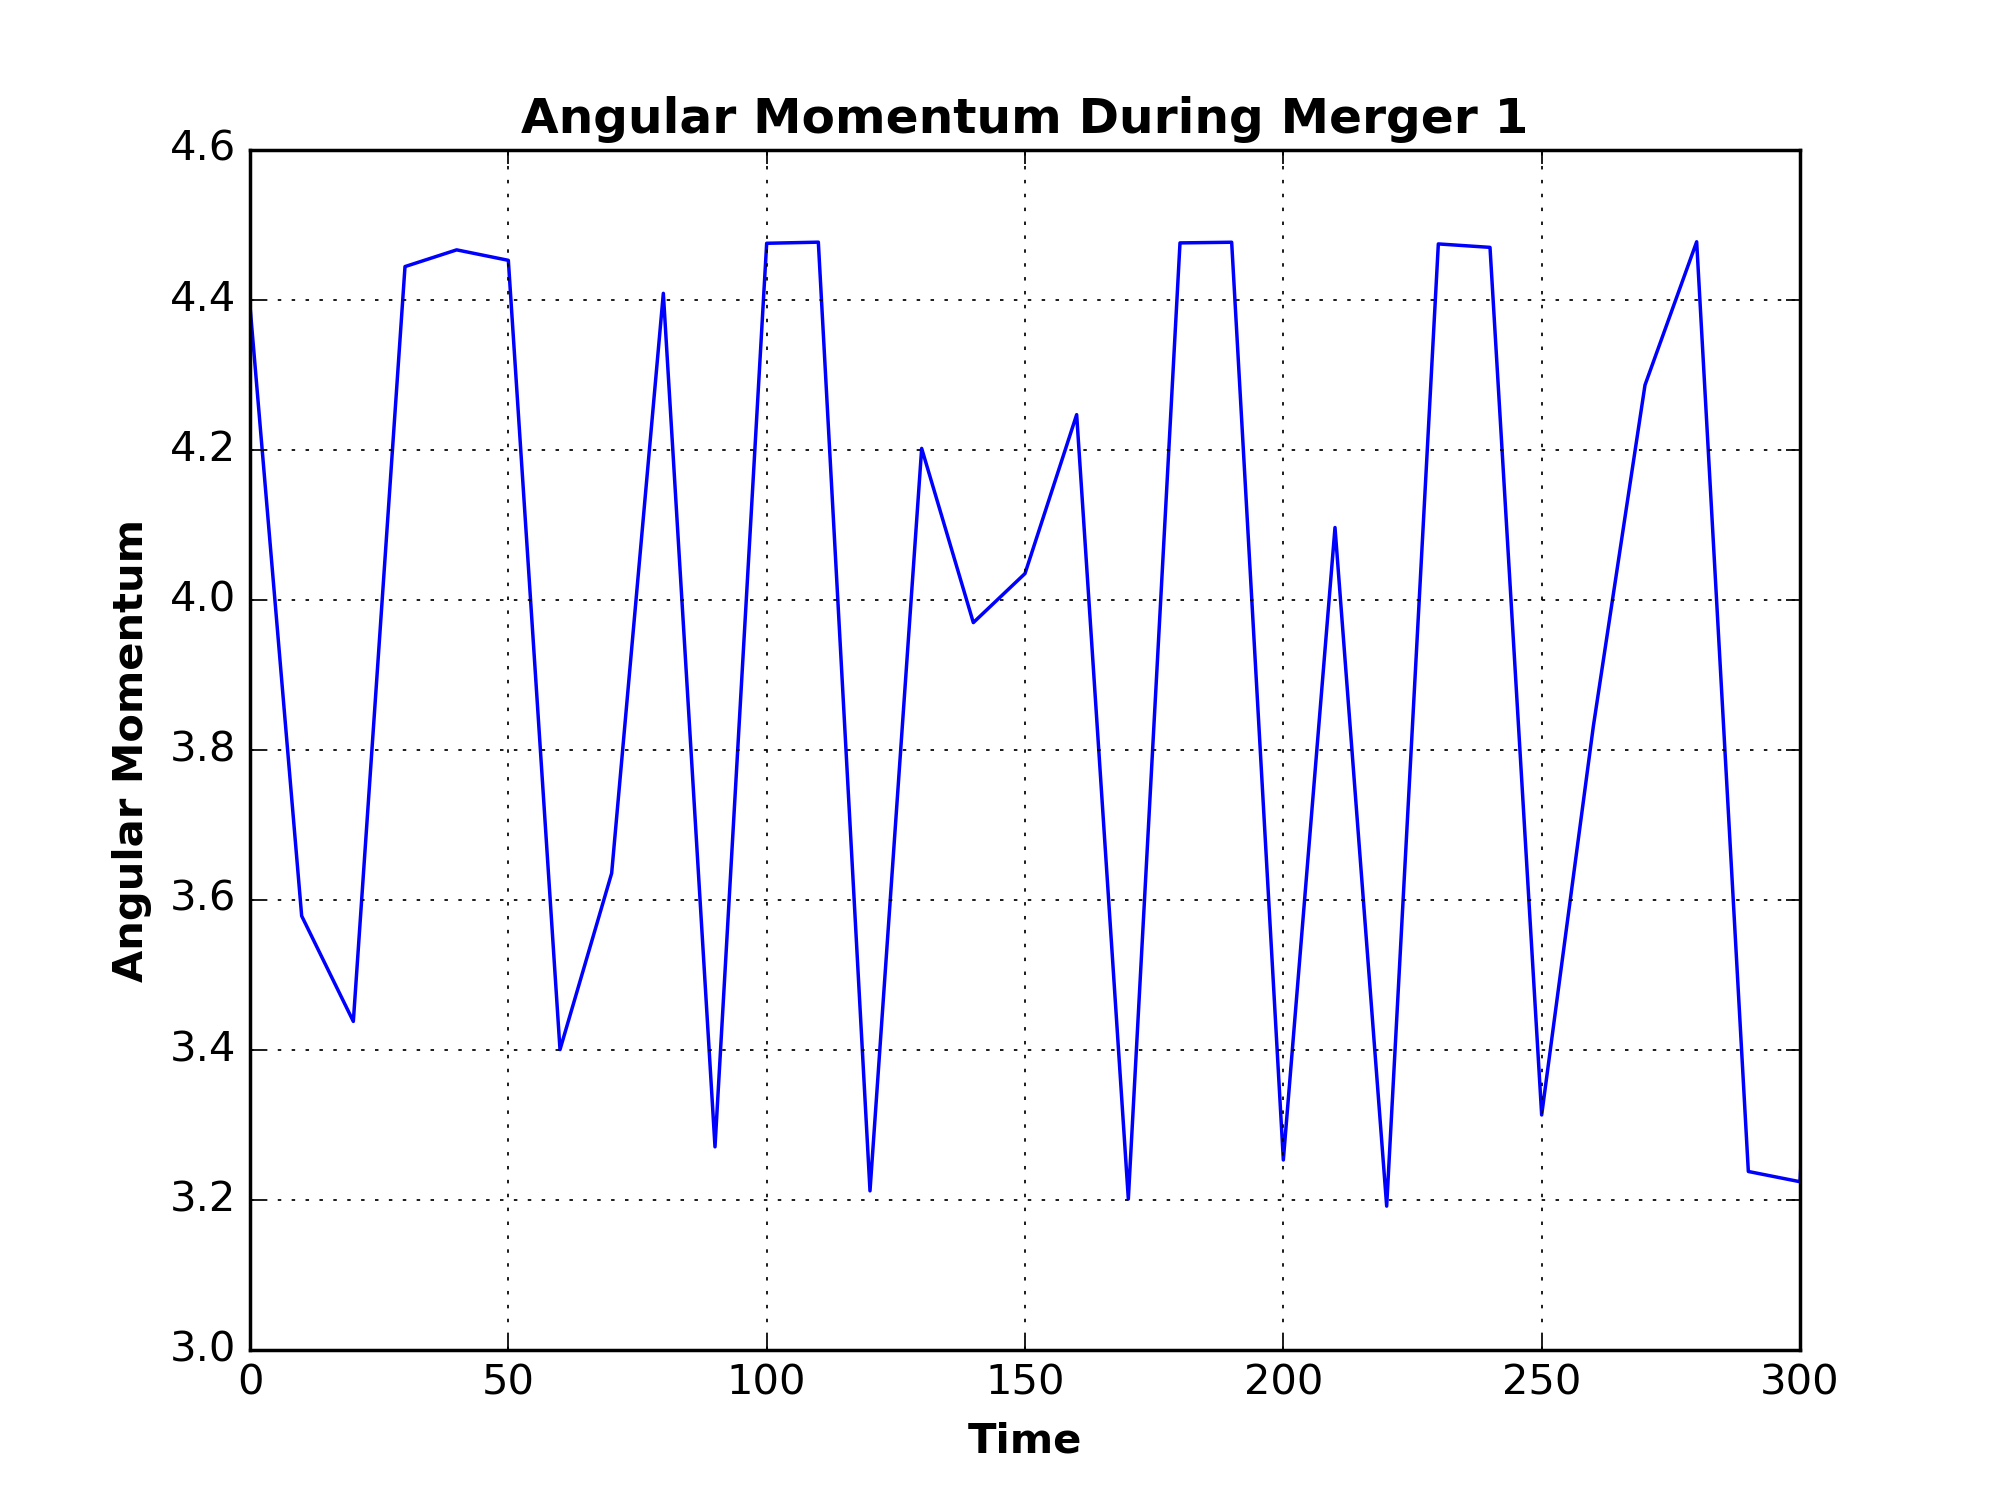
\includegraphics[width=\linewidth]{angular_momentum_merg13.png}
        \caption[]%
        {{The angular momentum during the first merger.}}
    
        \label{fig:ang_merger1}
    \end{subfigure} %'
    \hfill
    \begin{subfigure}[b]{.475\textwidth}
        \centering
        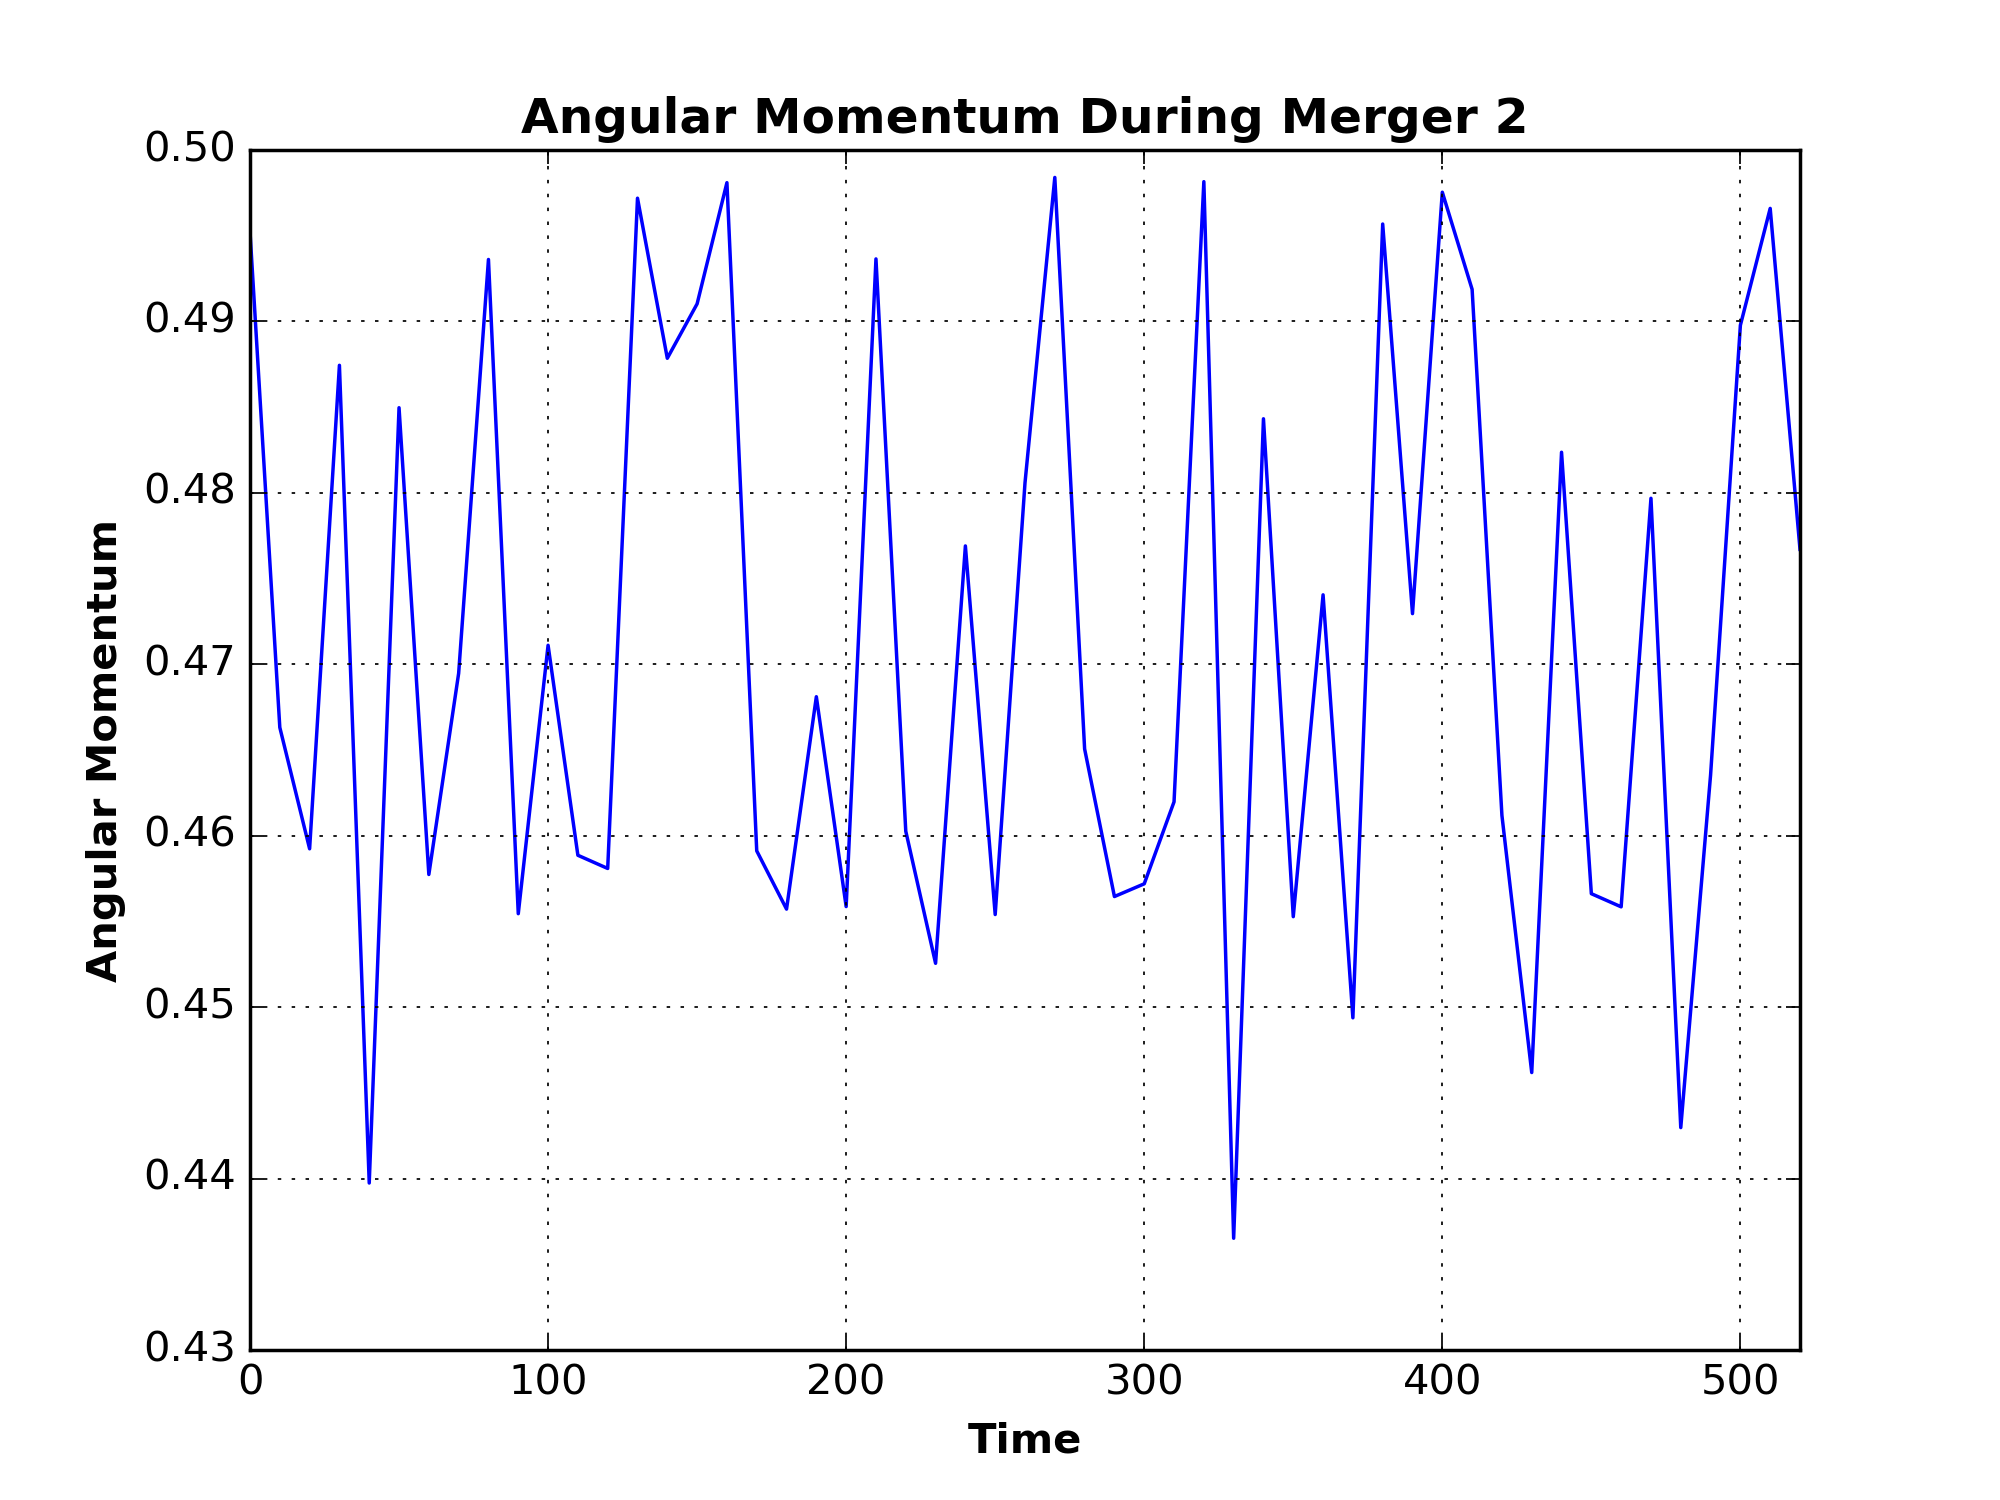
\includegraphics[width=\linewidth]{angular_momentum_merg21.png}
        \caption[]%
        {{The angular momentum during the second merger.}}
        \label{fig:ang_merger2} 
    \end{subfigure} %
    \caption[]
        {The plots above illustrate the total angular momentum during the duration of the mergers.} 
        \label{fig:angular_mmentum}
\end{figure}


Angular momentum was calculated by using the equation
\begin{equation}\label{eqn:angularmomentum_eqn}
    \vec{L} = \vec{r} \times m \vec{v},
\end{equation}
where $\vec{L}$ is the angular momentum, $\vec{r}$ is the averaged position of all of the particles, and $\vec{v}$ is the averaged velocity of all of the particles. By doing so, the plots in Figure~\ref{fig:angular_mmentum} were created that illustrate the total angular momentum of the two mergers.

\begin{figure}[H]
\centering 
    \begin{subfigure}[b]{.475\textwidth}
        \centering
        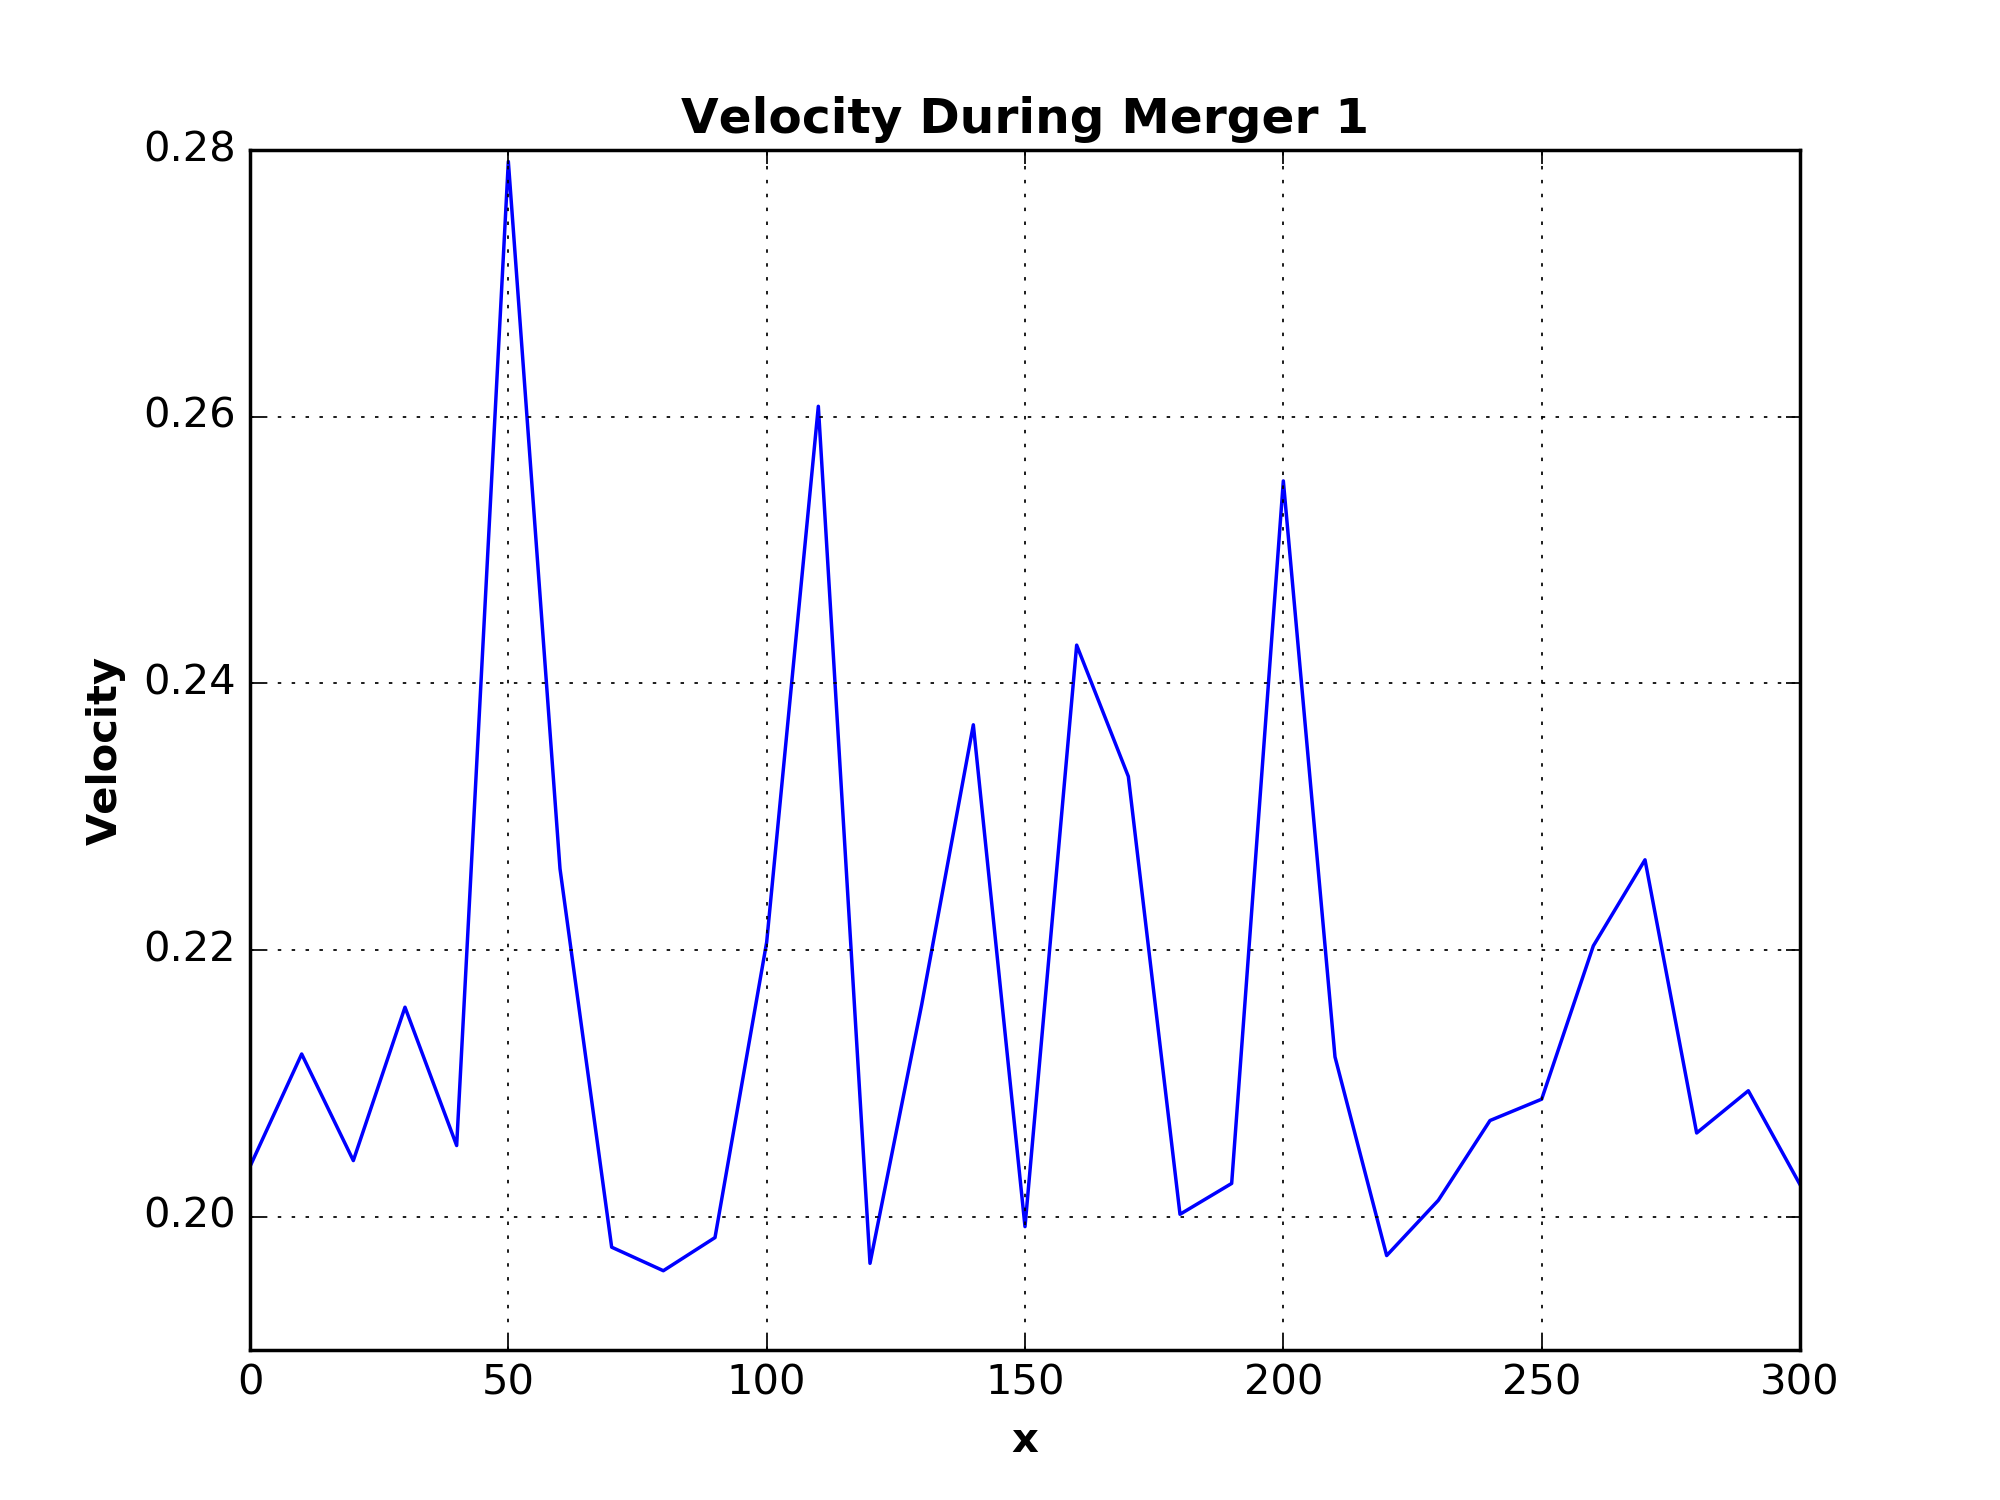
\includegraphics[width=\linewidth]{velocity_merger1.png}
        \caption[]%
        {{The velocity of the x-direction during the first merger.}}
    
        \label{fig:velcoity_merger1}
    \end{subfigure} %'
    \hfill
    \begin{subfigure}[b]{.475\textwidth}
        \centering
        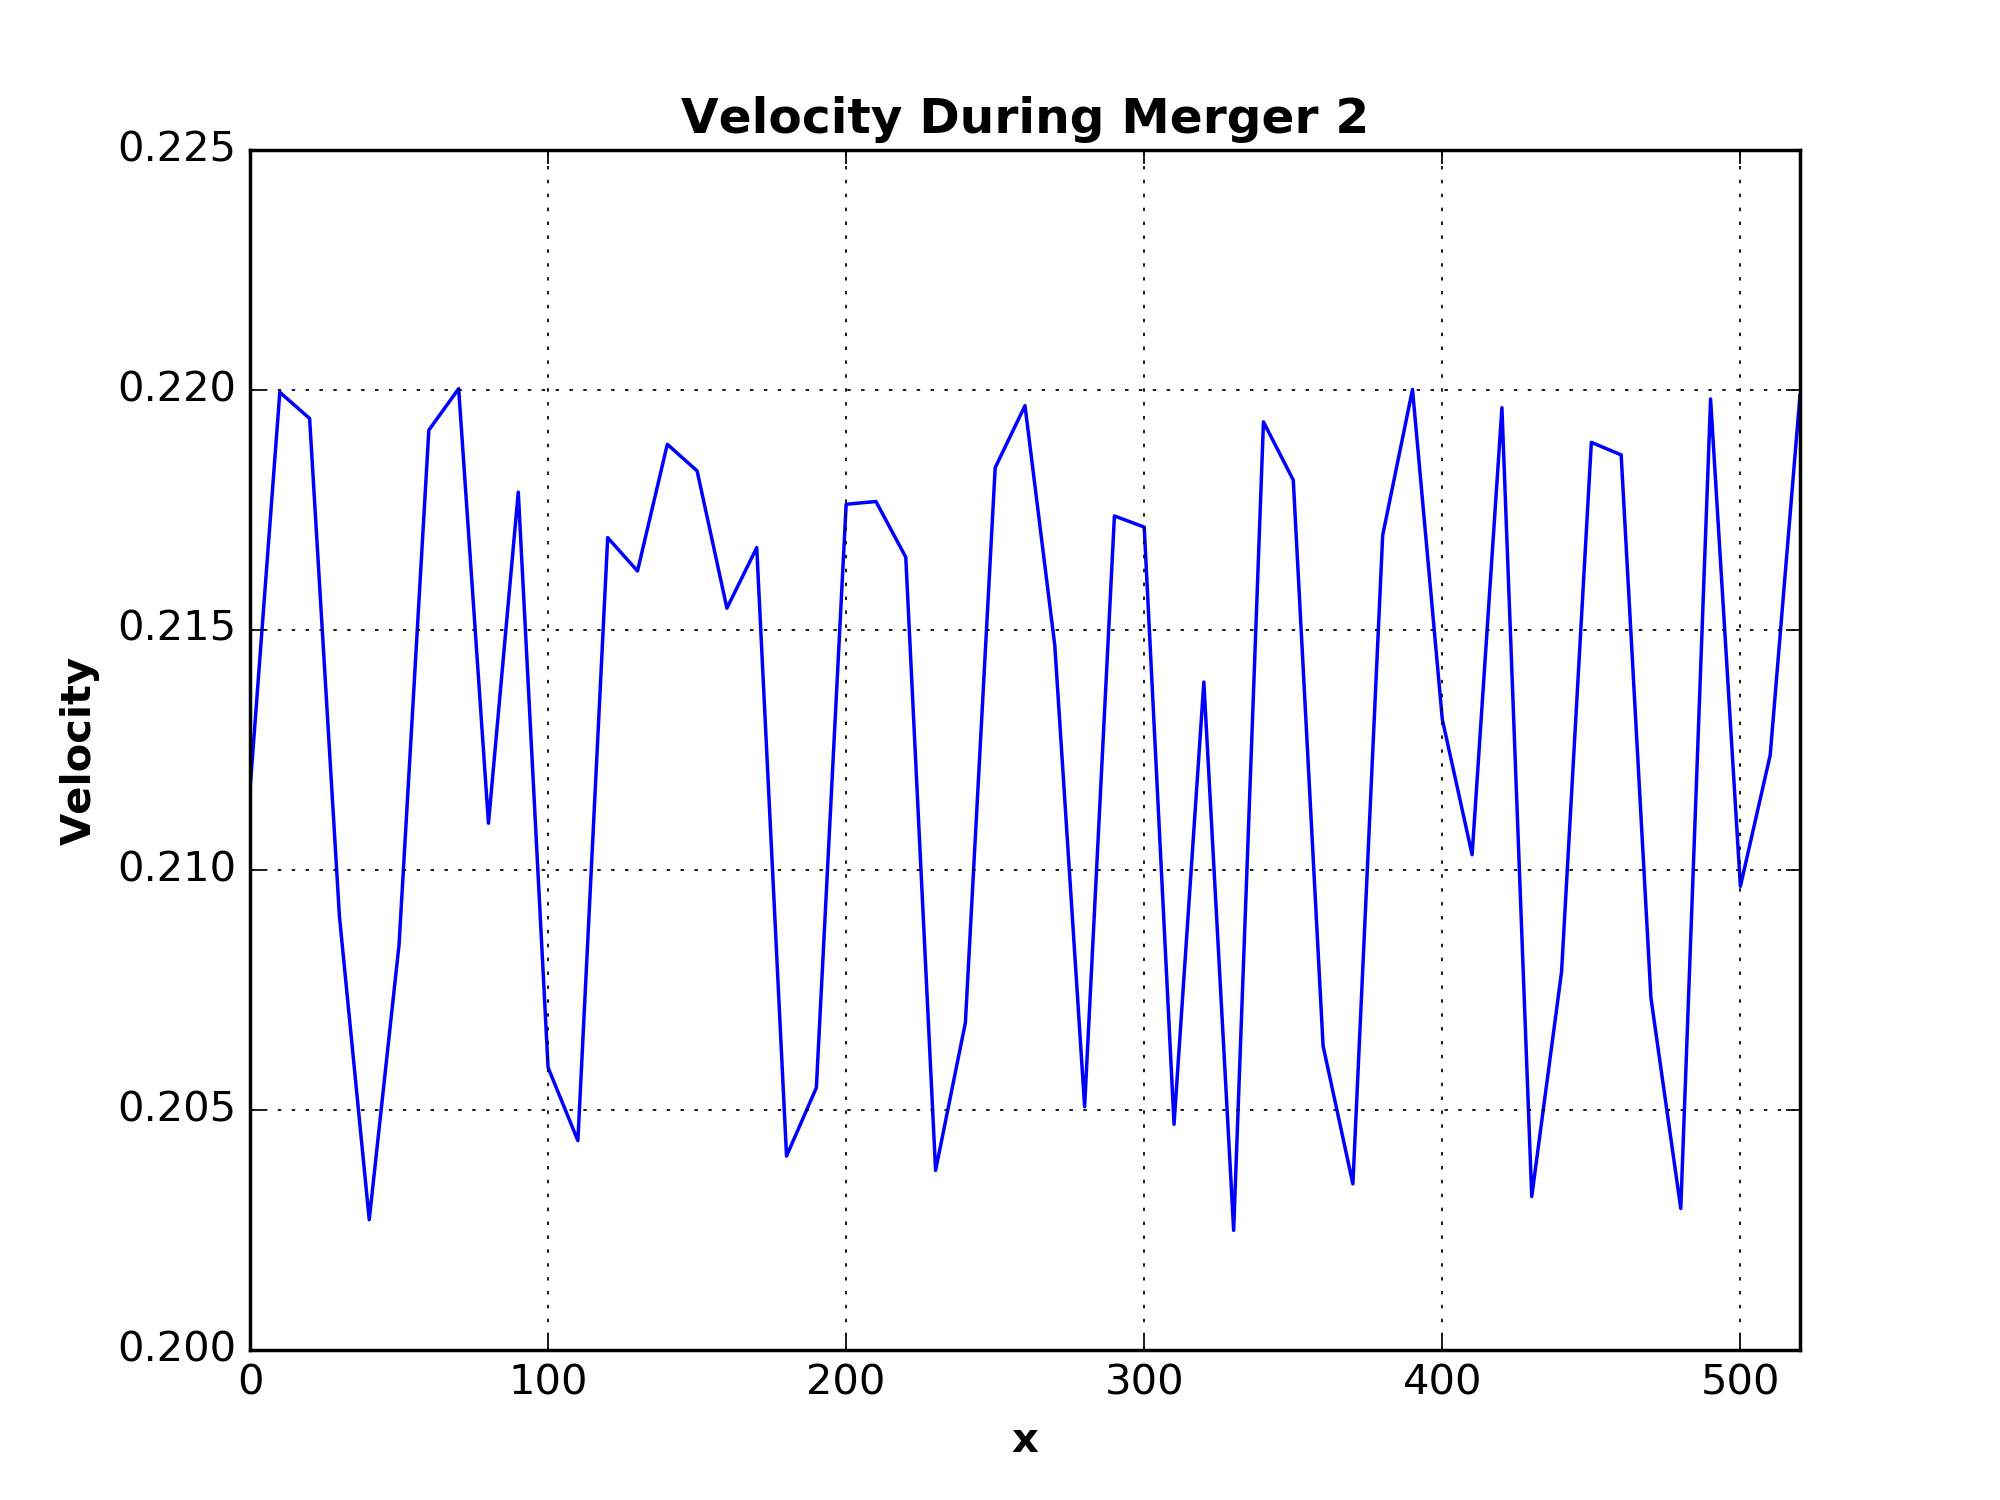
\includegraphics[width=\linewidth]{velocity_merger2.png}
        \caption[]%
        {{The velocity of the x-direction during the second merger.}}
        \label{fig:velocity_merger2}
    \end{subfigure} %
    \caption[]
        {The plots above illustrate the velocity in the x-direction during the duration of the mergers.} 
        \label{fig:velocity_of_mergers}
\end{figure}

Because there were three velocities for the x-, y-, and z-direction, only the velocity in the x-direction was used for this illustration of how the velocities were effected by the mergers. By plotting the average velocity in the x-direction for each time step against time, one can visualize the nature of the particles during the merger. This can be seen in Figure~\ref{fig:velocity_of_mergers} above.





\section*{Results} \label{sec:Results}
\addcontentsline{toc}{section}{Results}

The results of the two different mergers summarized in Table~\ref{tab:Models} are discussed. 

\subsection*{Merger 1}
\addcontentsline{toc}{subsection}{Merger 1}


\begin{figure}[H]
        \centering
        \begin{subfigure}[b]{0.48\textwidth}
            \centering
            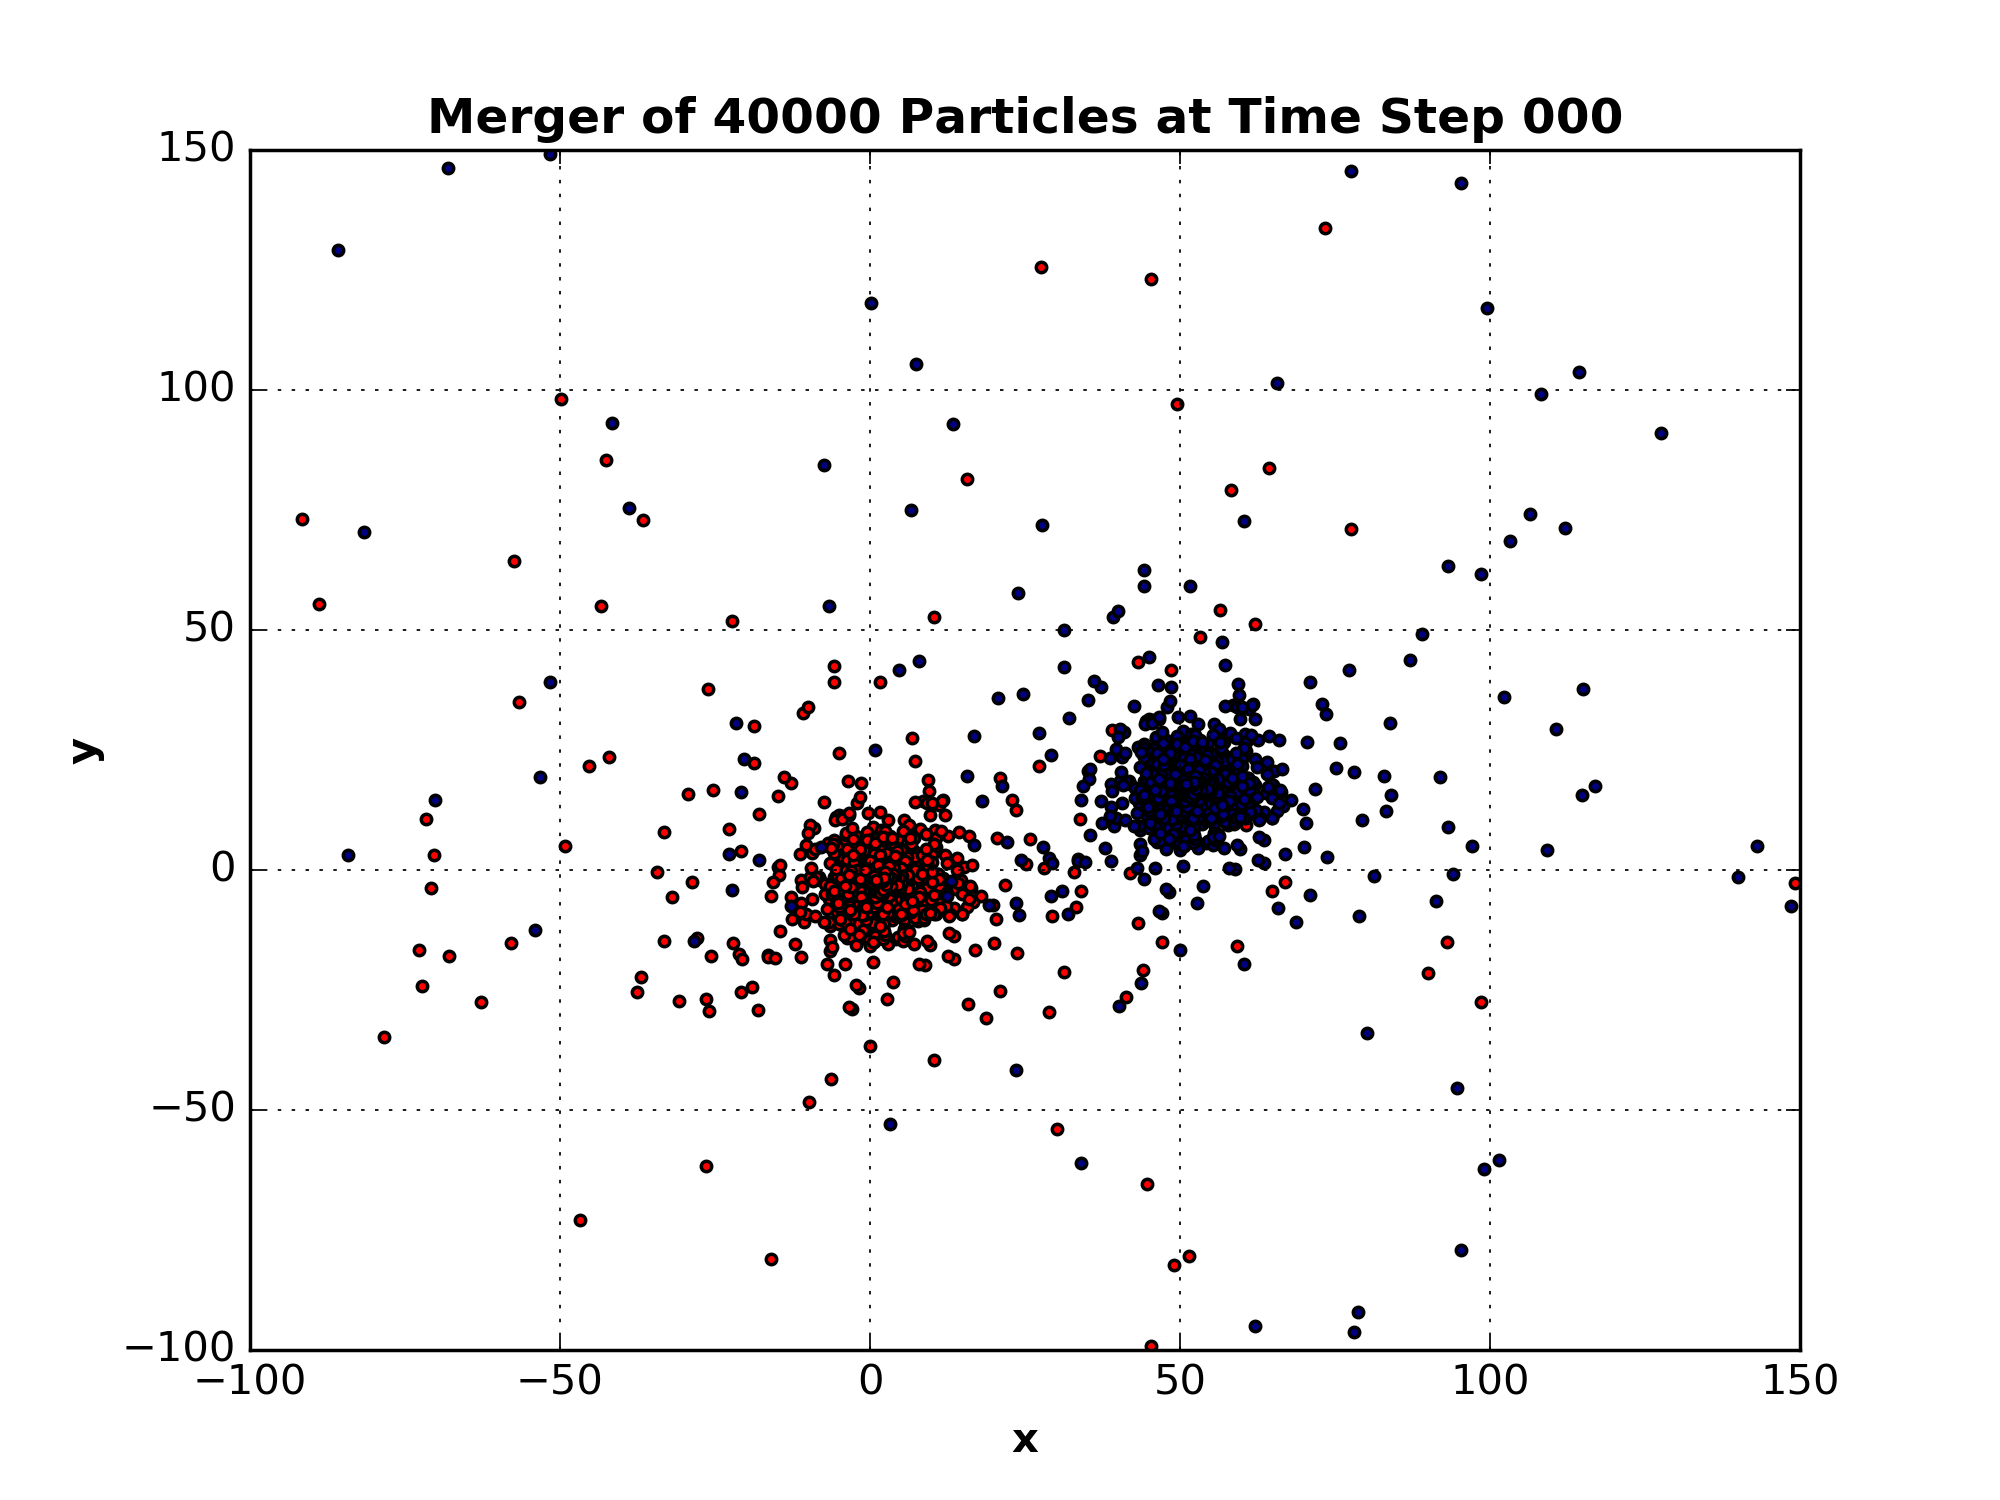
\includegraphics[width=\linewidth]{mergert000.png}
            \caption[]%
            {{\small The two elliptical galaxies separated by an x-shift of $50$ and y-shift of $20$.}}    
            \label{fig:merger1_t00}
        \end{subfigure}
        \hfill
        \begin{subfigure}[b]{0.48\textwidth}  
            \centering 
            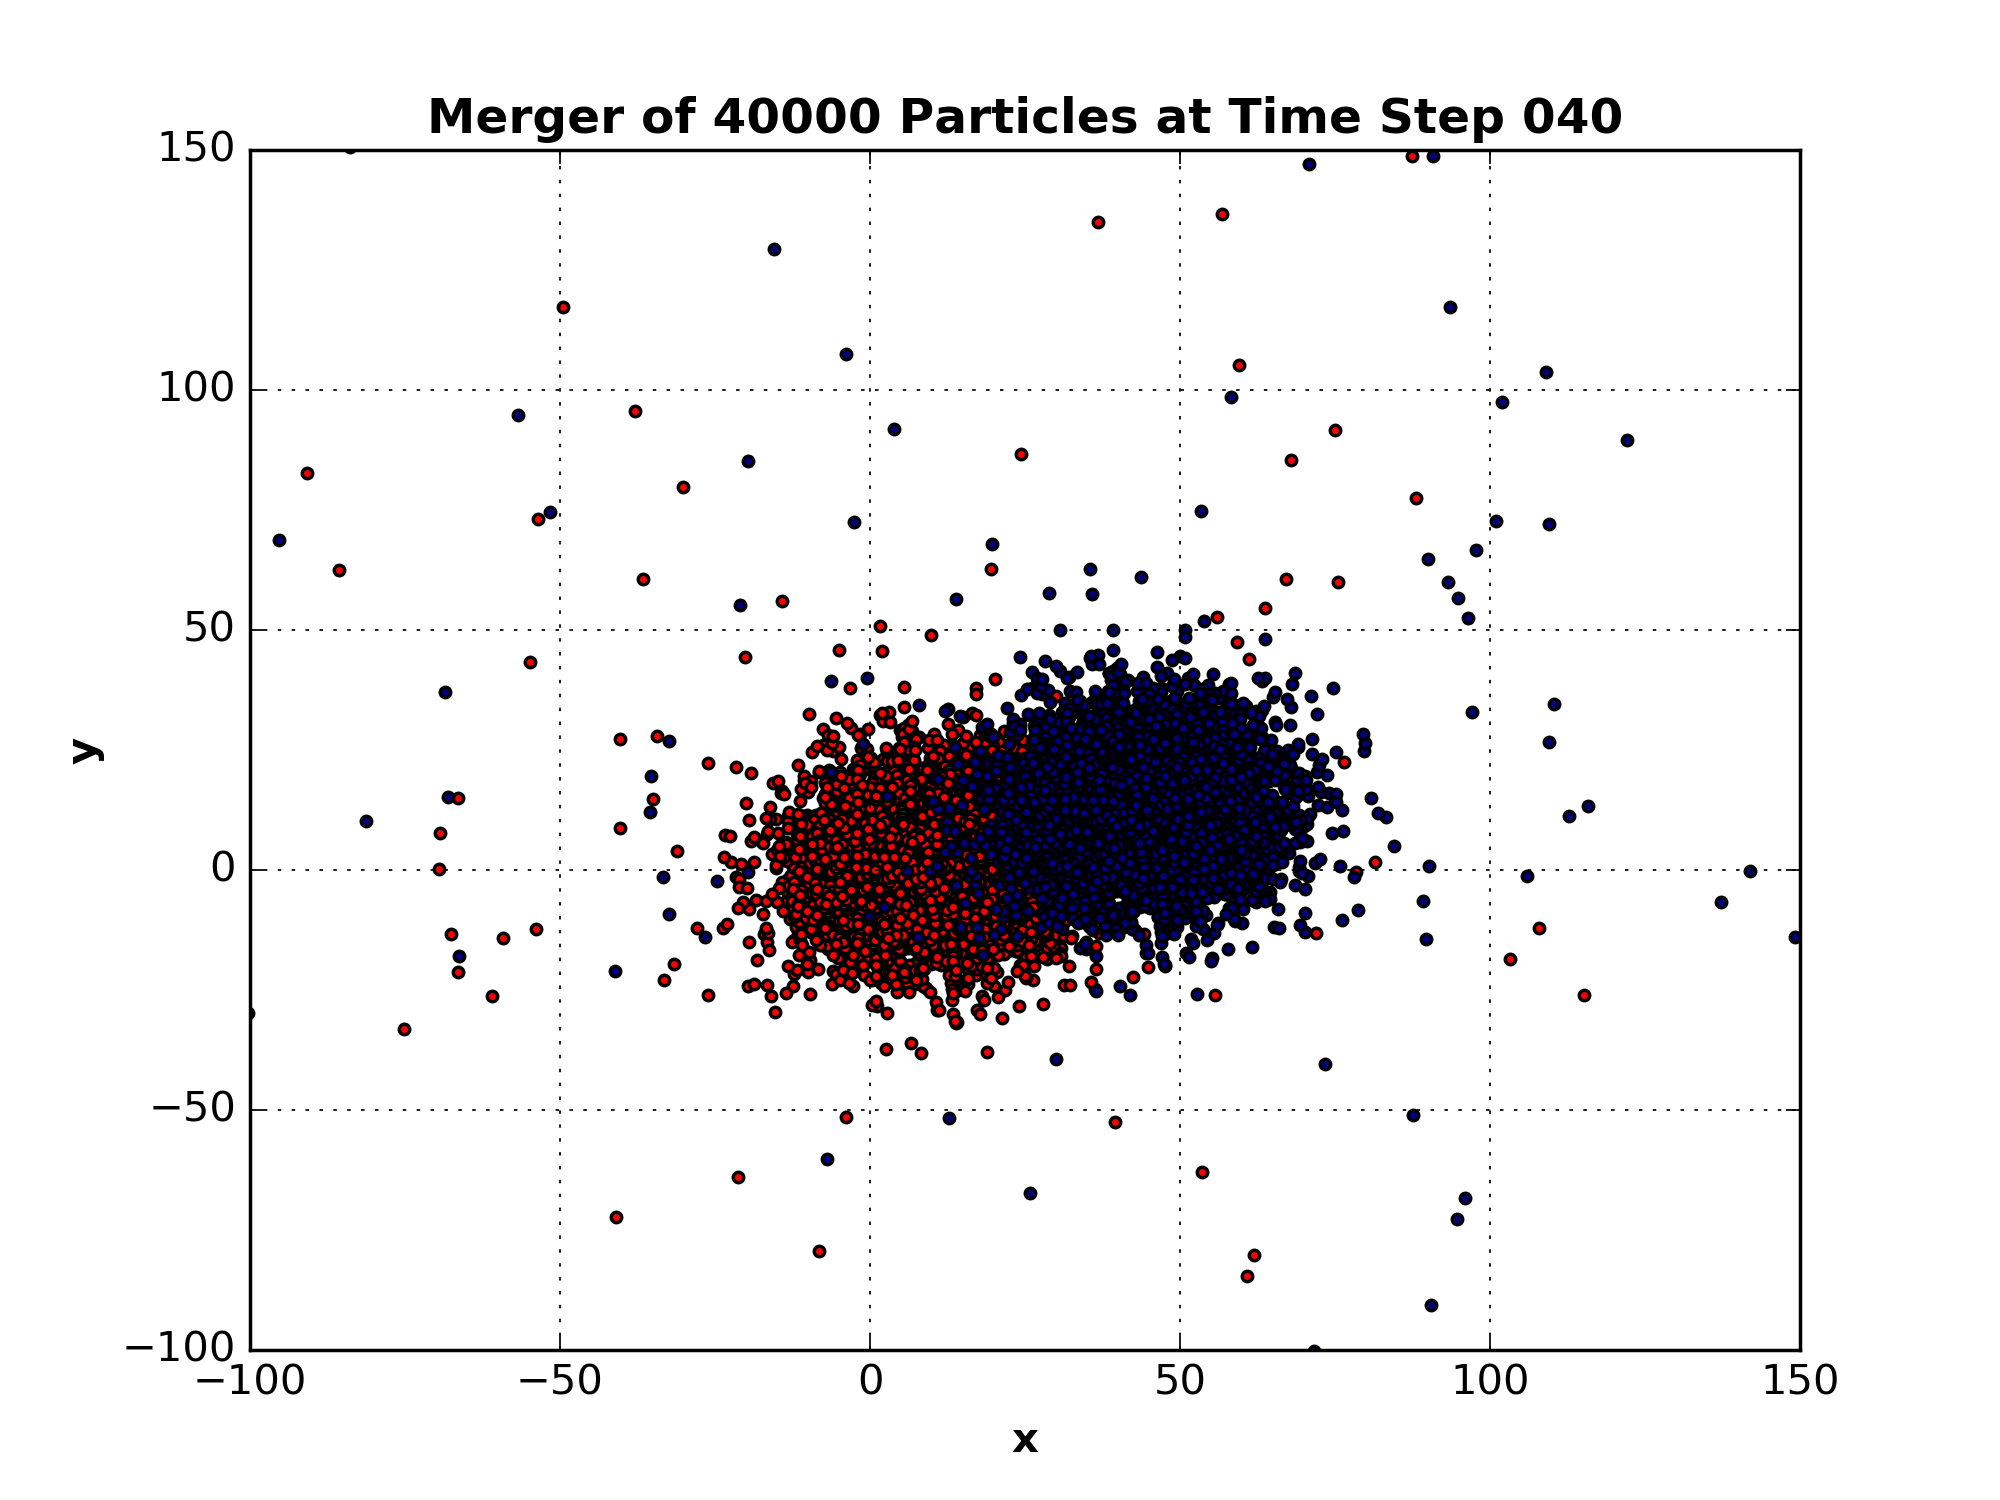
\includegraphics[width=\linewidth]{mergert040.png}
            \caption[]%
            {{\small The initial merging of the two elliptical galaxies at a time step of $40$.}}    
            \label{fig:merger1_t040}
        \end{subfigure}
        \vskip\baselineskip
        \begin{subfigure}[b]{0.48\textwidth}   
            \centering 
            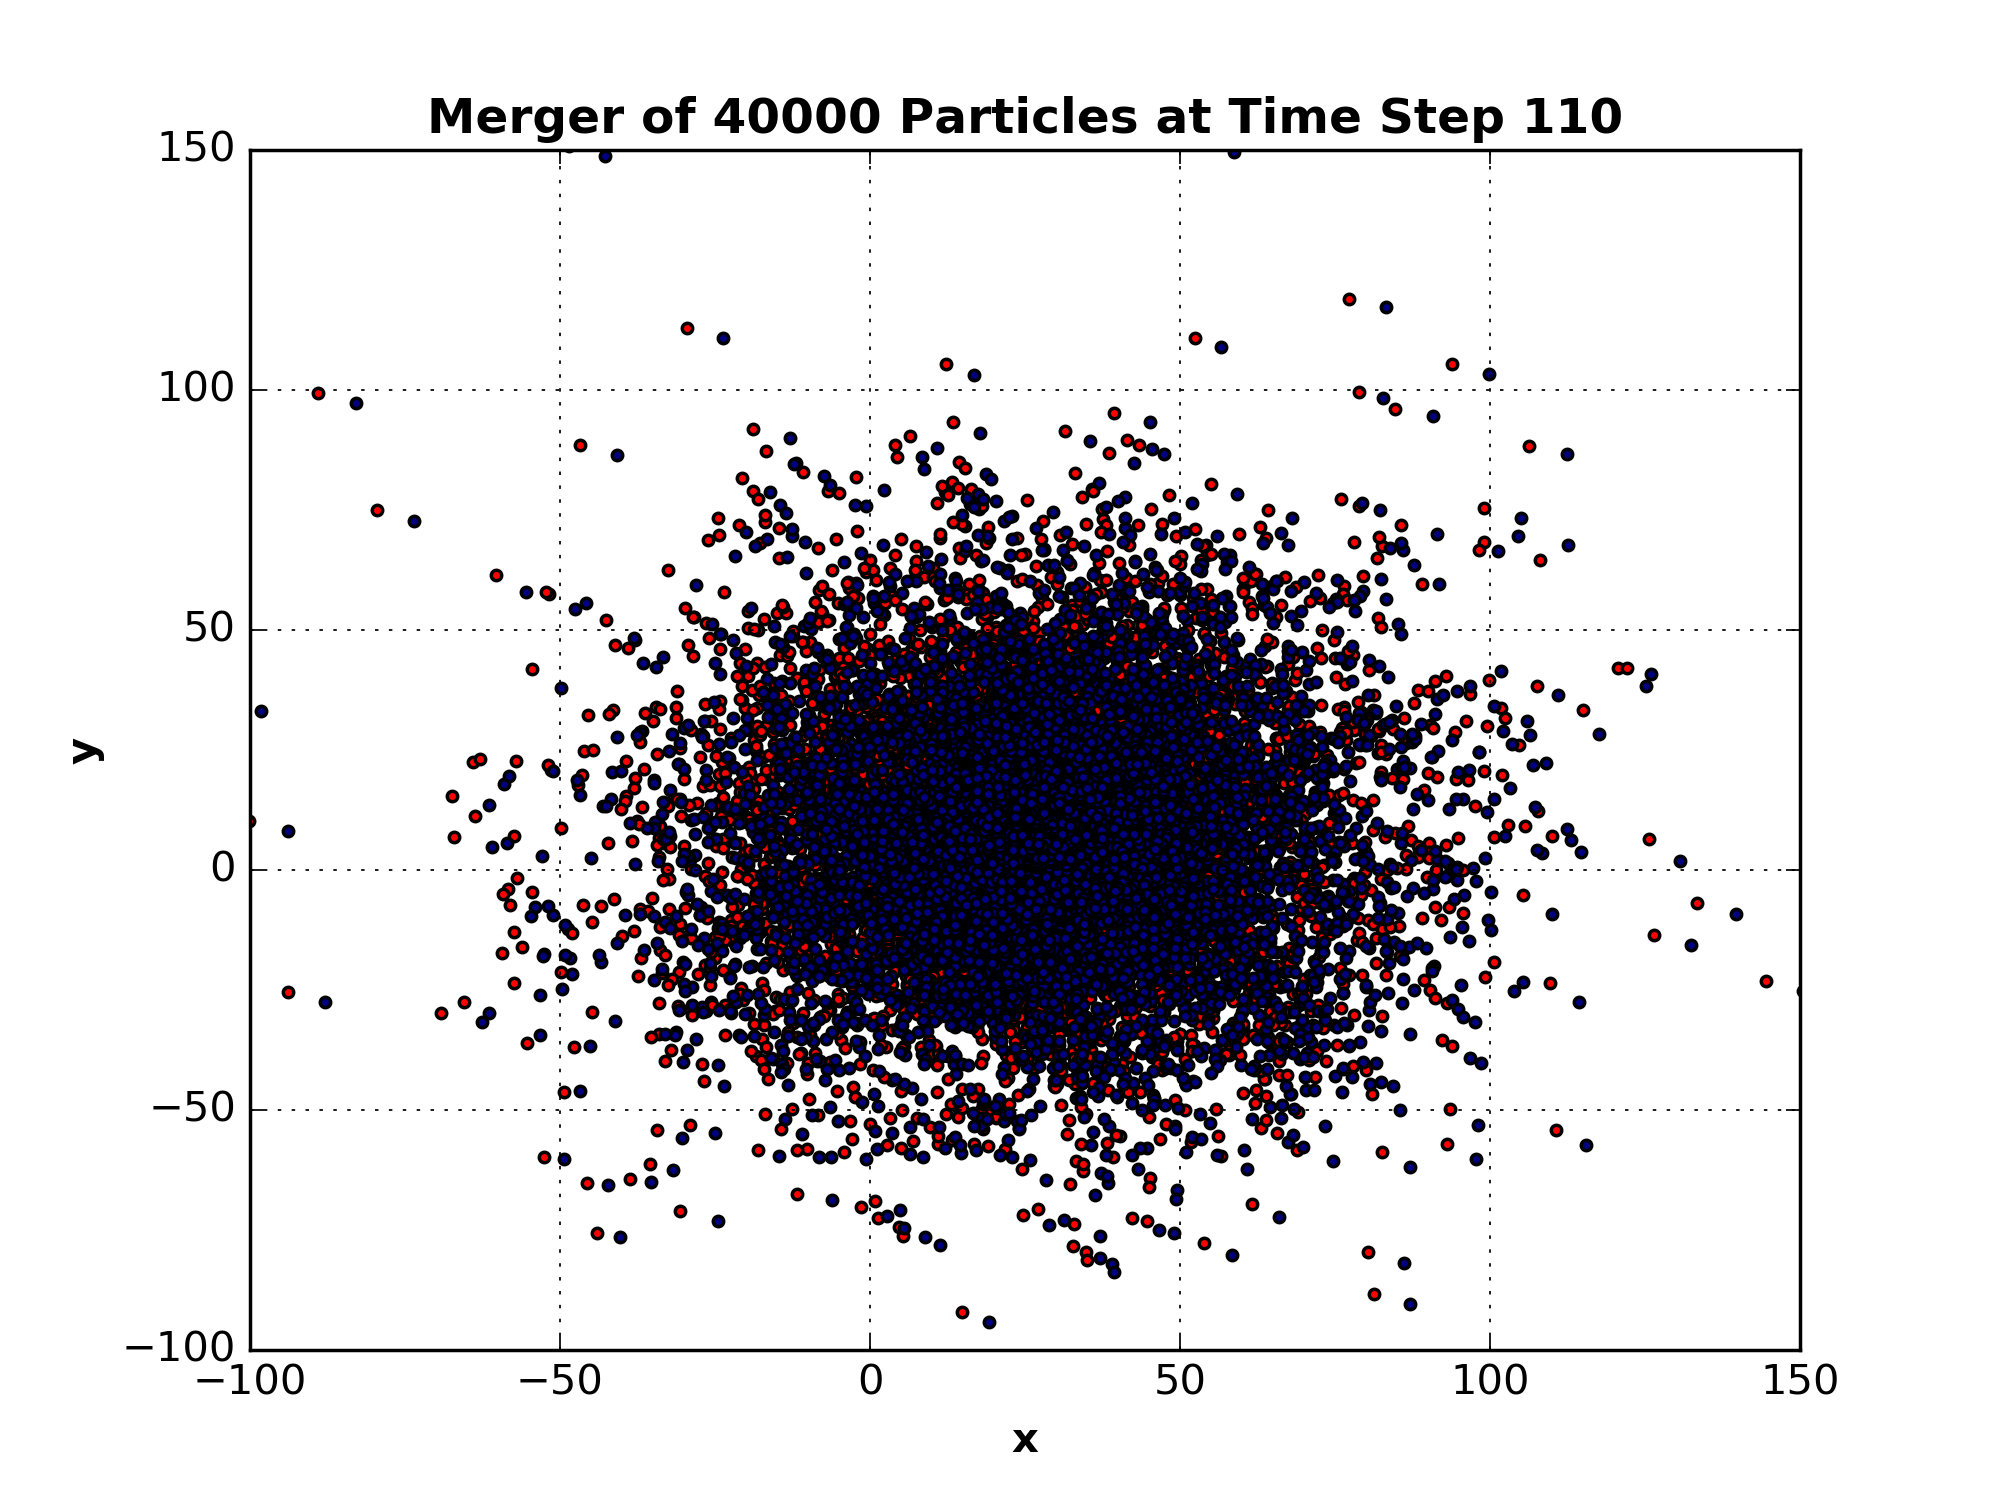
\includegraphics[width=\linewidth]{mergert110.png}
            \caption[]%
            {{\small The two elliptical galaxies completely merged at a time step of $110$.}}    
            \label{fig:merger1_t110}
        \end{subfigure}
        \quad
        \begin{subfigure}[b]{0.48\textwidth}   
            \centering 
            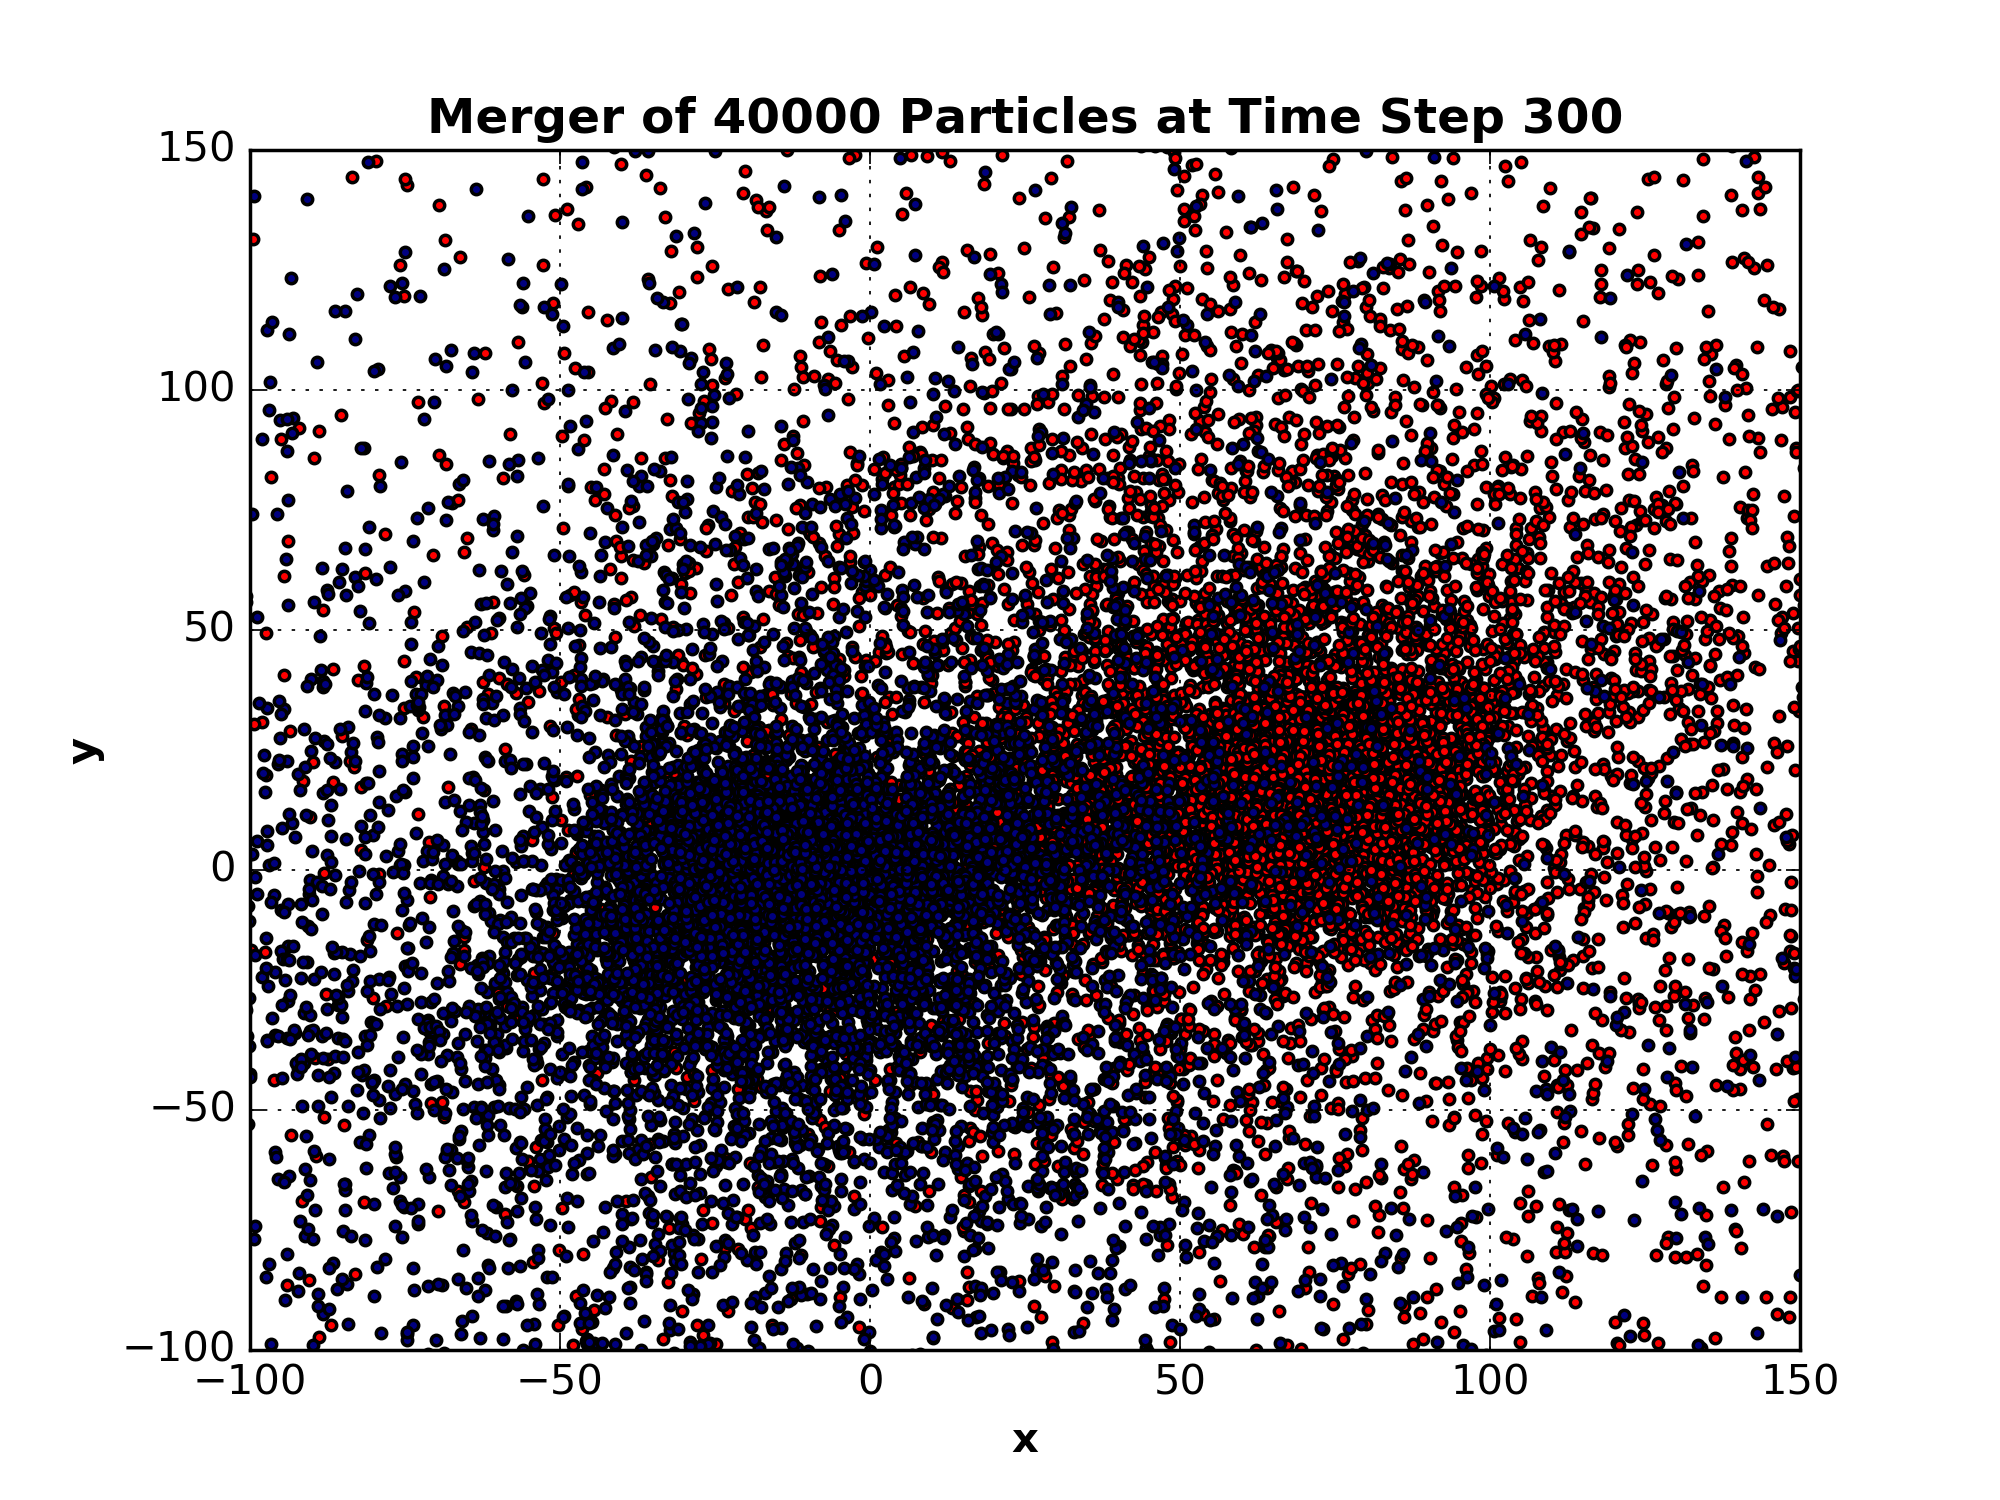
\includegraphics[width=\textwidth]{mergert300.png}\
            \caption[]%
            {{\small The two elliptical galaxies after the merger at a time step of $300$.}}
            \label{fig:merger1_t300}
        \end{subfigure}
        \caption[]
        {The plots above illustrate the first merger.}
        \label{fig:merger1}
    \end{figure}
    
  Figure~\ref{fig:merger1} shows the merging process of the two elliptical galaxies. As seen, even with an initial offset in the y-direction, the galaxies did not spiral into one another; rather, they just collided head-on.
  
\begin{figure}[H]
\centering 
    \begin{subfigure}[b]{.475\textwidth}
        \centering
        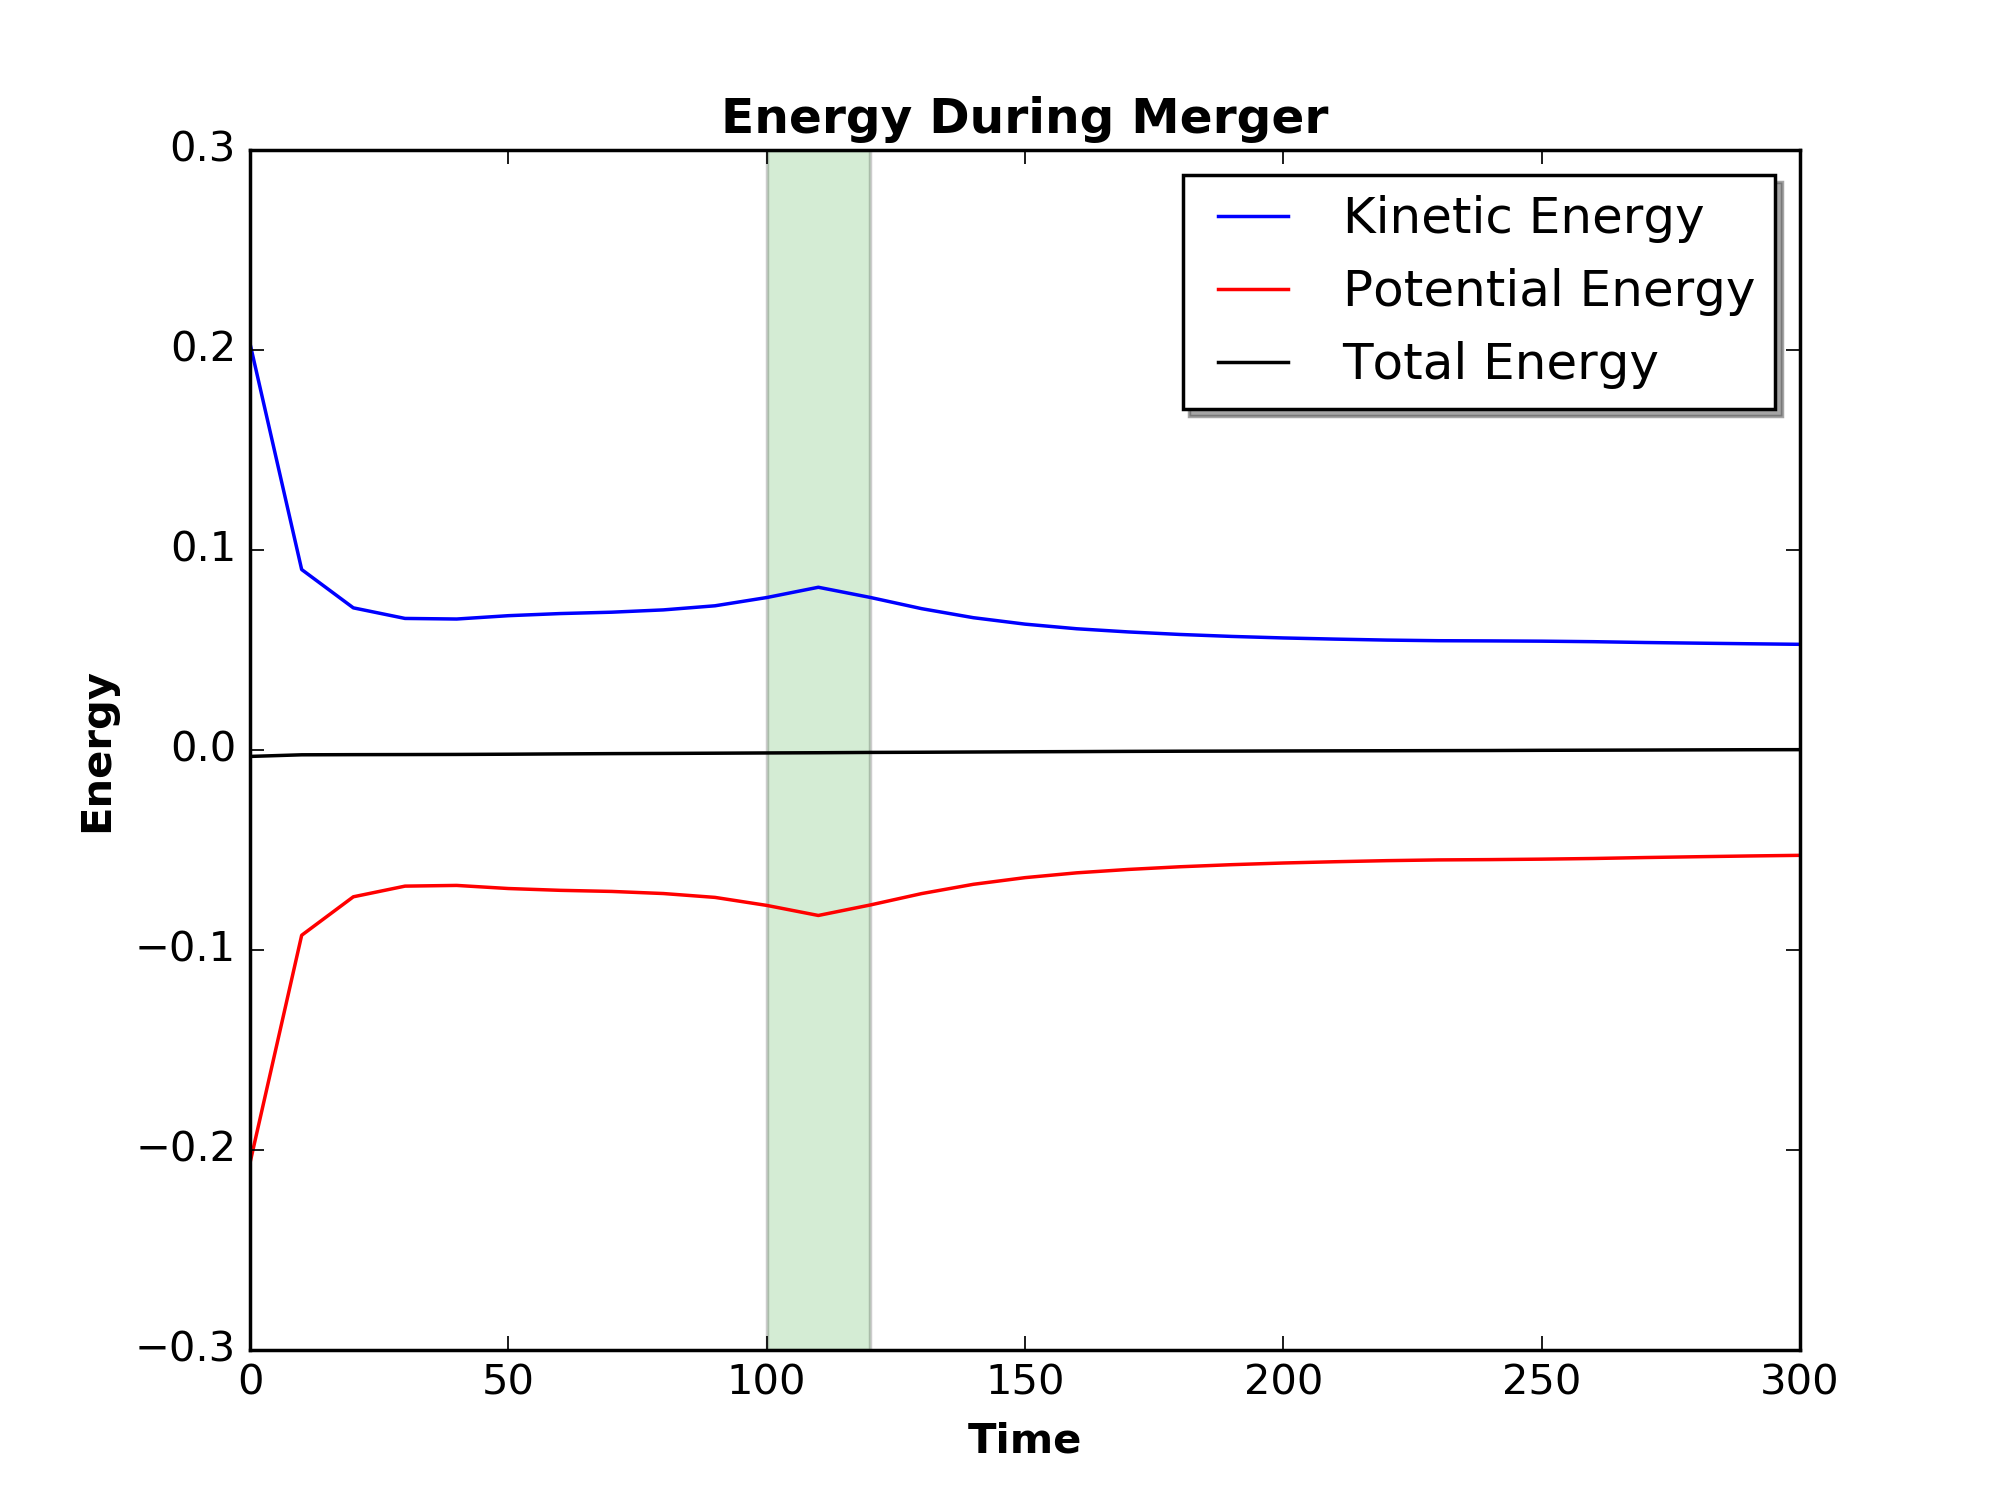
\includegraphics[width=\linewidth]{Energy_of_merger-model1.png}
        \caption[]%
        {{Kinetic energy, potential energy, and total energy versus time.}}
        
        \label{fig:totalenergy}
    \end{subfigure} %'
    \hfill
    \begin{subfigure}[b]{.475\textwidth}
        \centering
        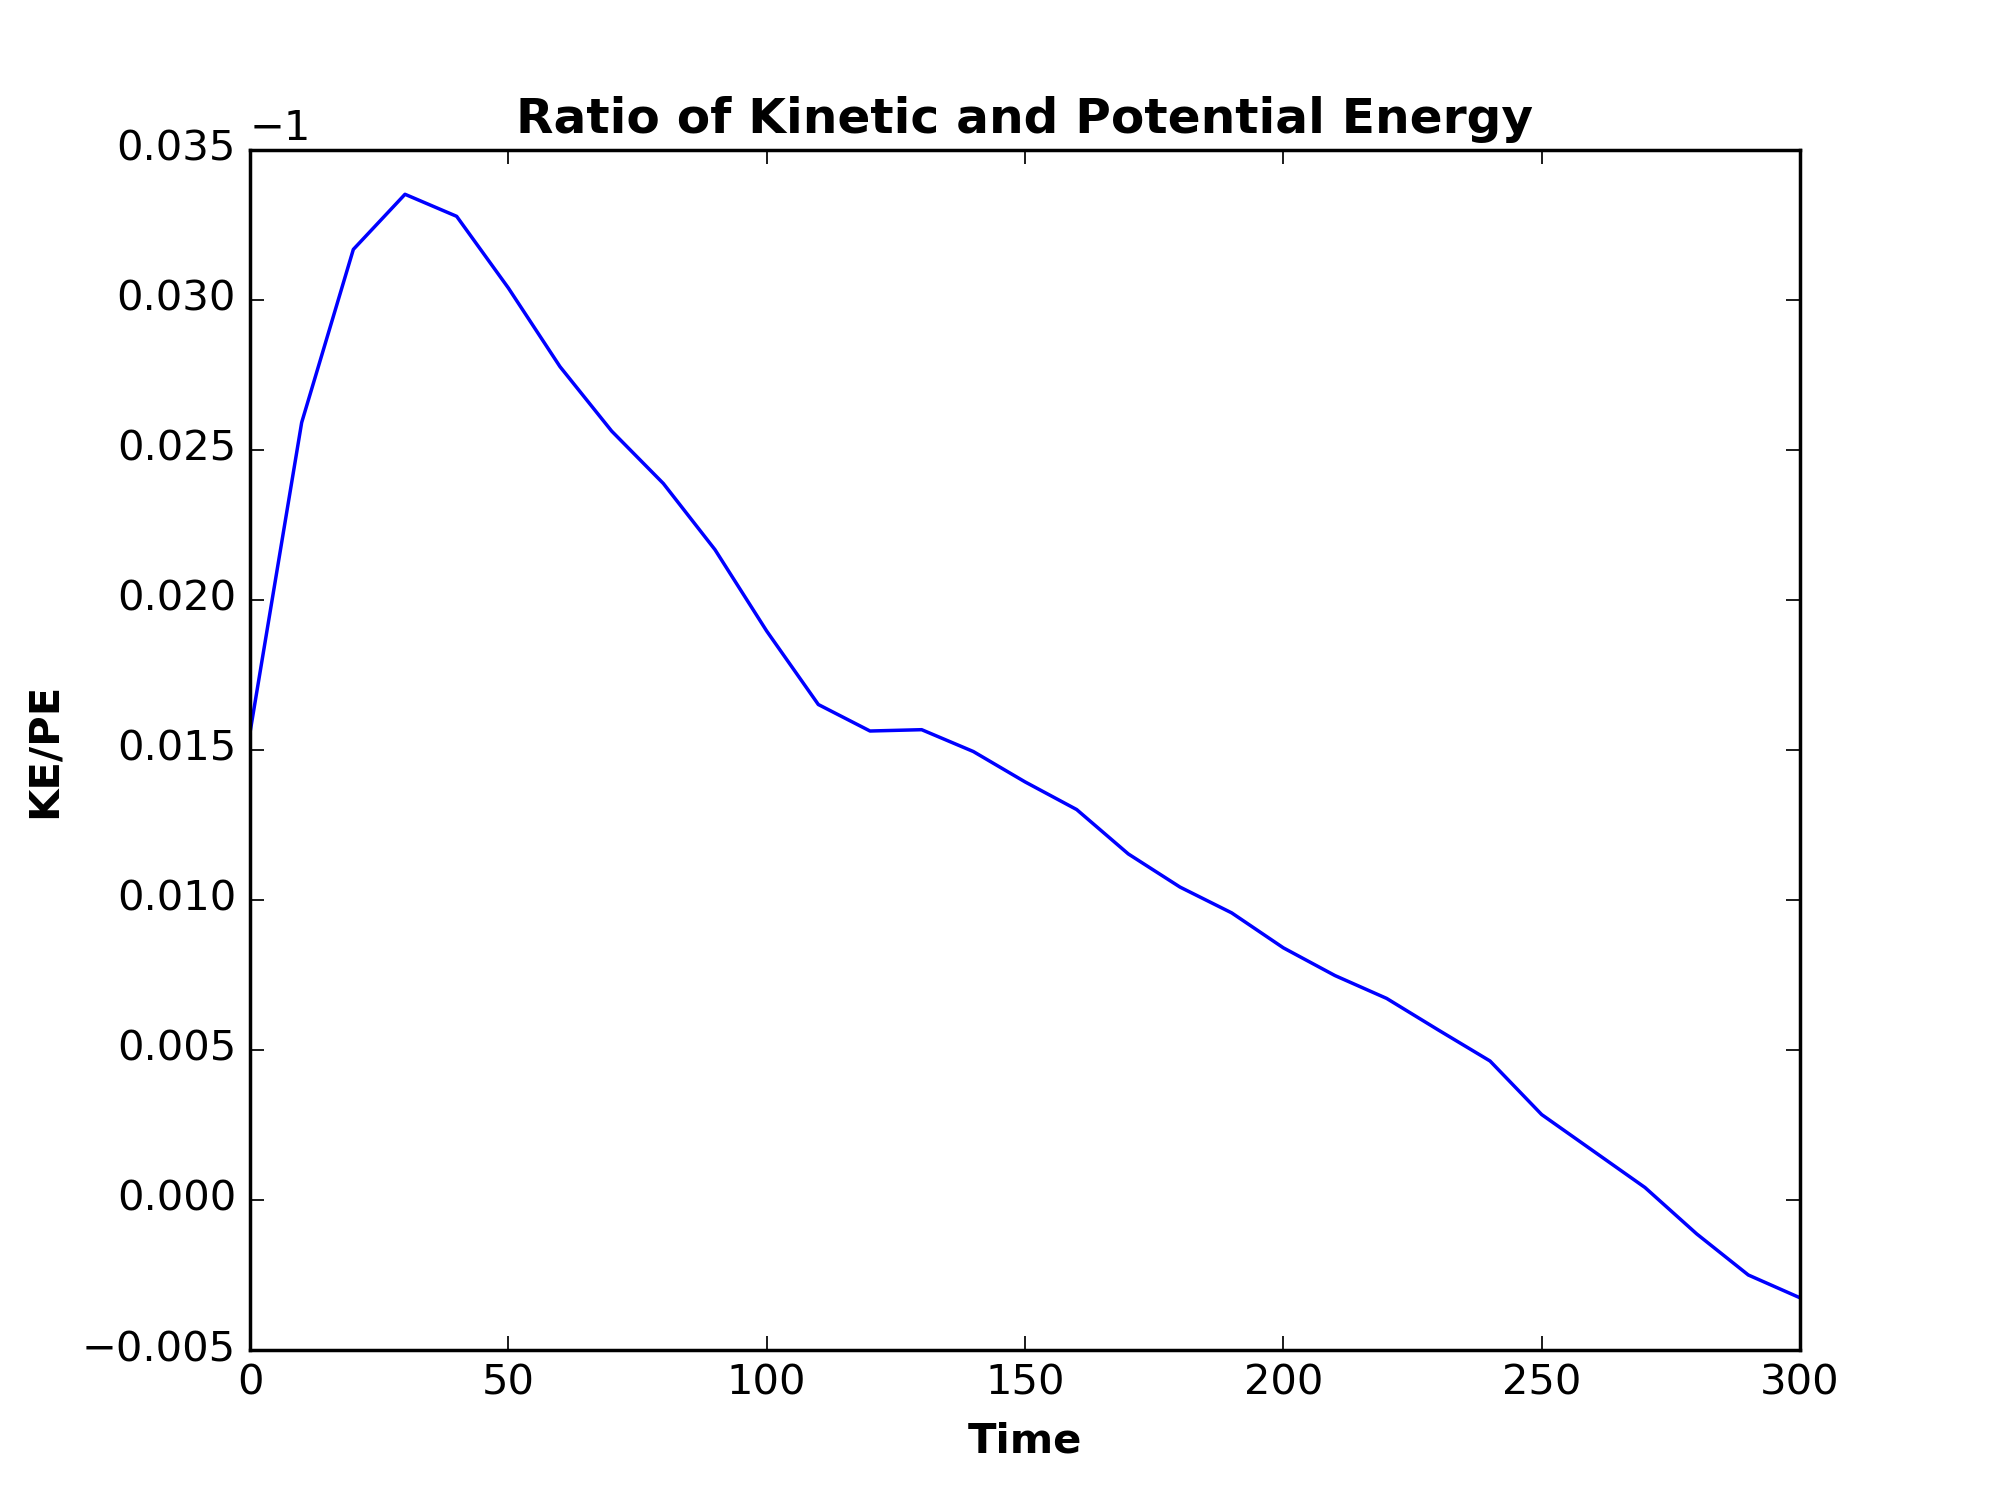
\includegraphics[width=\linewidth]{ratioofkineticandpotential_mod1.png}
        \caption[]%
        {{The ratio between kinetic and potential energy versus time.}}
        \label{fig:ratiomerger1}
    \end{subfigure} %
    \caption[]
        {The plots above illustrate the energy change during the merger highlighted in Figure~\ref{fig:merger1}. The green shaded area in Figure~\ref{fig:totalenergy} highlights a particular perturbation in the energy of the system corresponding to time step $110$ seen in Figure~\ref{fig:merger1_t110}.} 
        \label{fig:energyofmerger1}
\end{figure}

Figure~\ref{fig:energyofmerger1} above illustrates the energy during the merger process seen in Figure~\ref{fig:merger1}. Something interesting to note is the slight perturbation (highlighted in green) seen in the curves of kinetic and potential energy in Figure~\ref{fig:totalenergy}. This area corresponds to the merger sequence of Figure~\ref{fig:merger1_t110}. This time step happens well after the initial start of the merger; thus, something is occurring at this time step that increases the kinetic energy and decreases the potential energy of the system. Perhaps this is when the merger becomes complete.

\subsection*{Merger 2}
\addcontentsline{toc}{subsection}{Merger 2}


\begin{figure}[H]
        \centering
        \begin{subfigure}[b]{0.48\textwidth}
            \centering
            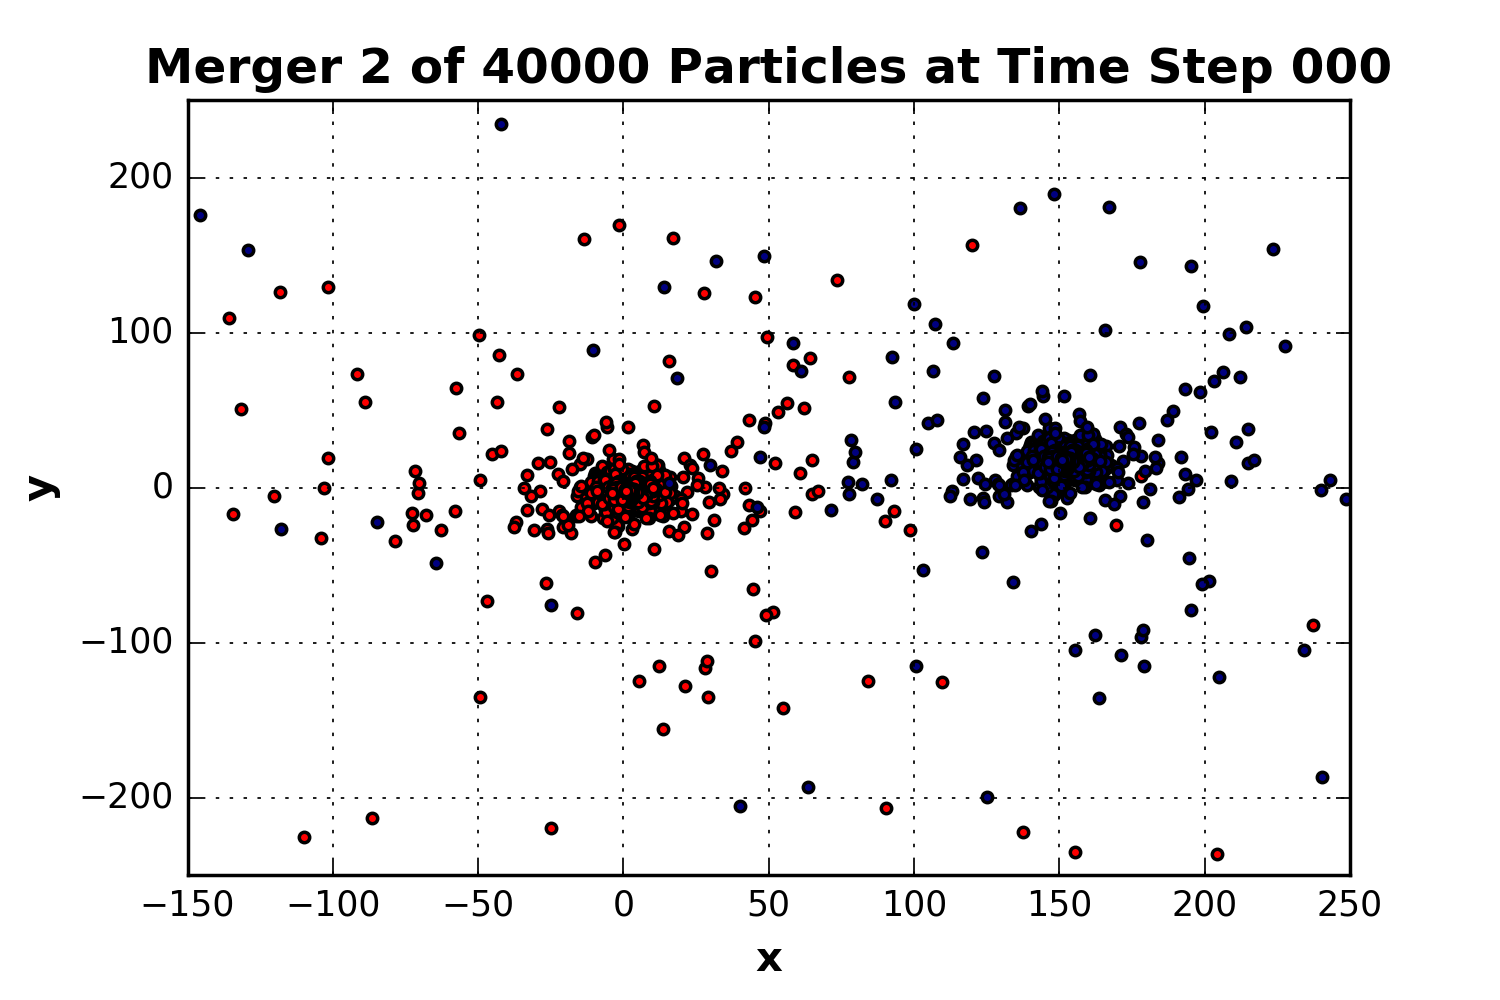
\includegraphics[width=\linewidth]{merger2t000.png}
            \caption[]%
            {{\small The two elliptical galaxies separated by an x-shift of $150$ and y-shift of $20$.}}    
            \label{fig:merger2_t00}
        \end{subfigure}
        \hfill
        \begin{subfigure}[b]{0.48\textwidth}  
            \centering 
            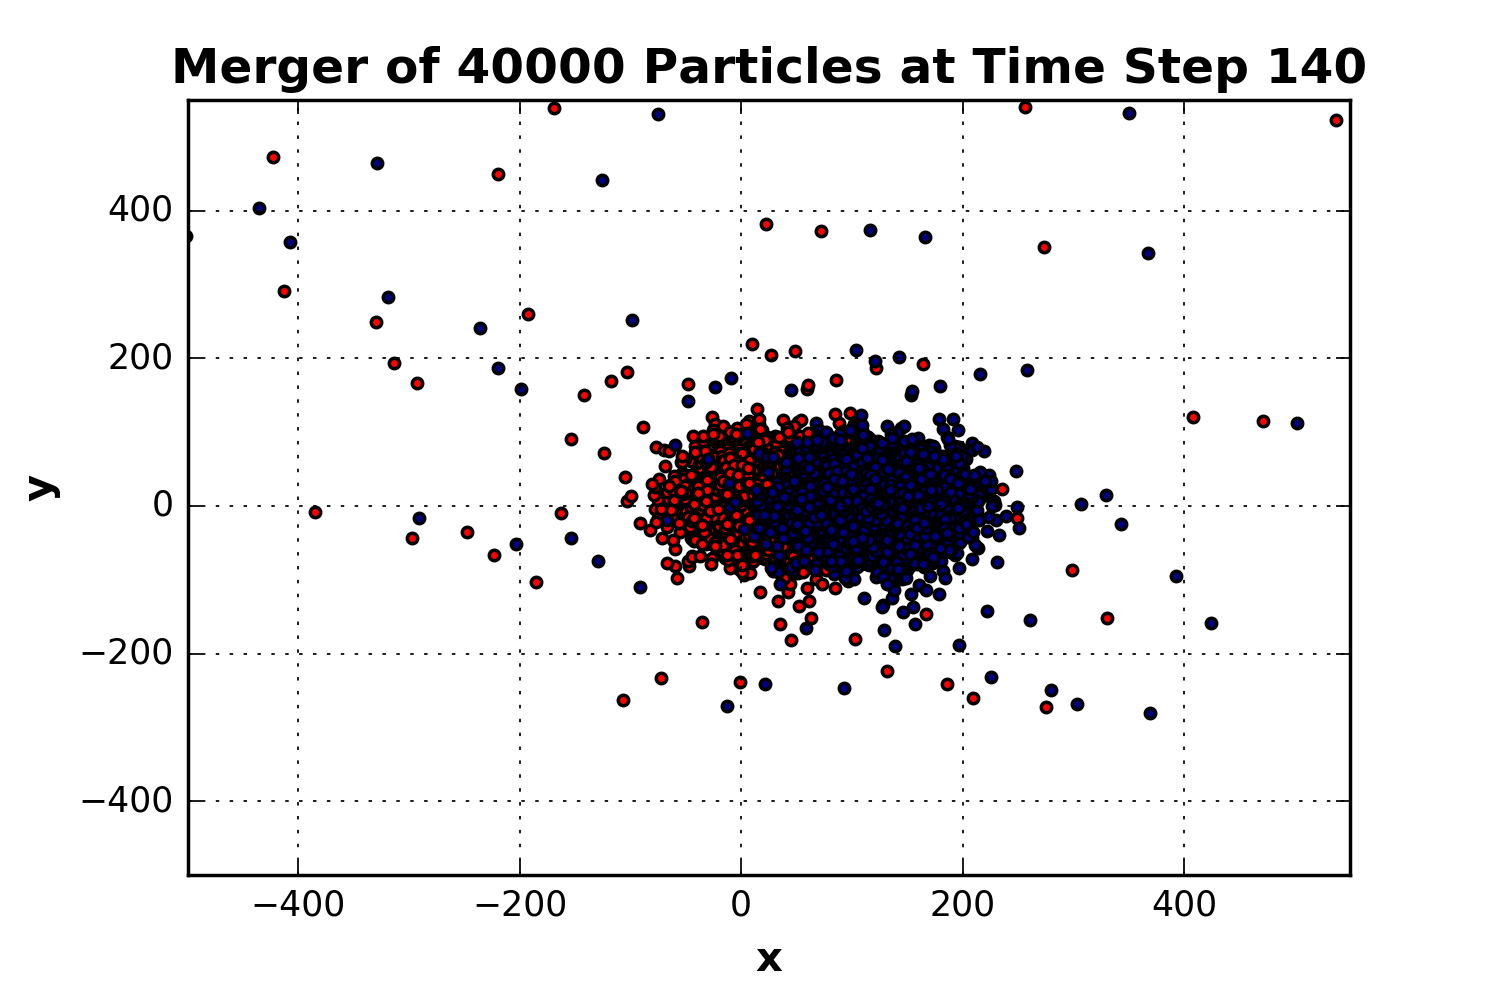
\includegraphics[width=\linewidth]{merger2_t140.png}
            \caption[]%
            {{\small The two elliptical galaxies merging at a time step of $140$.}}    
            \label{fig:merger2_t140}
        \end{subfigure}
        \vskip\baselineskip
        \begin{subfigure}[b]{0.48\textwidth}   
            \centering 
            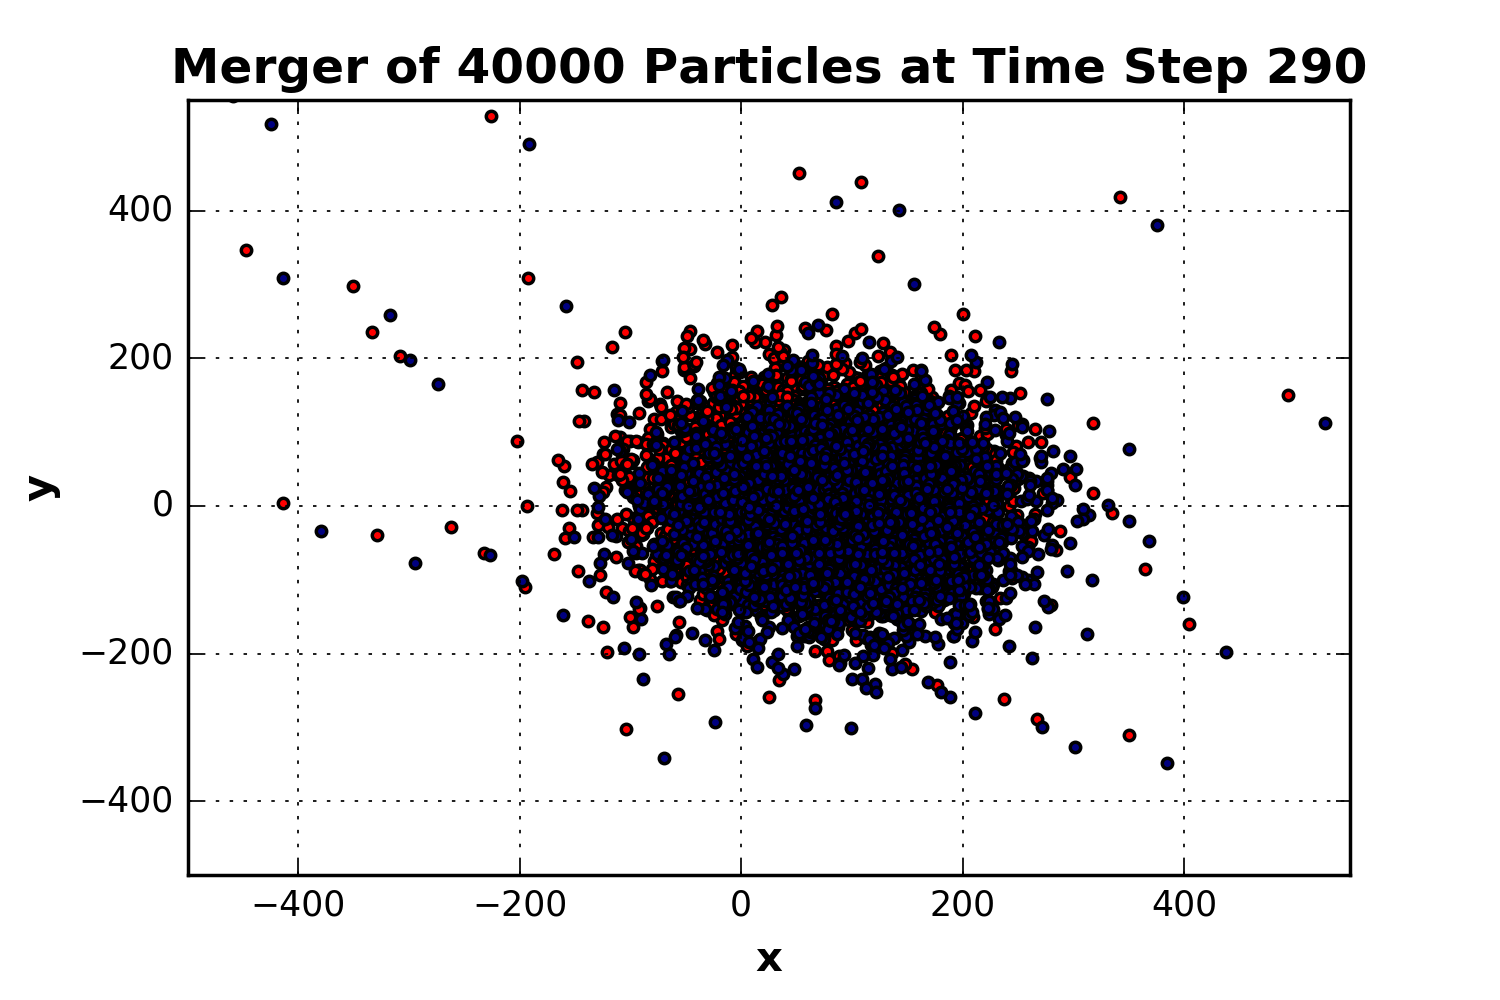
\includegraphics[width=\linewidth]{merger2_t290.png}
            \caption[]%
            {{\small The two elliptical galaxies completely merged at a time step of $290$.}}    
            \label{fig:merger2_t200}
        \end{subfigure}
        \quad
        \begin{subfigure}[b]{0.48\textwidth}   
            \centering 
            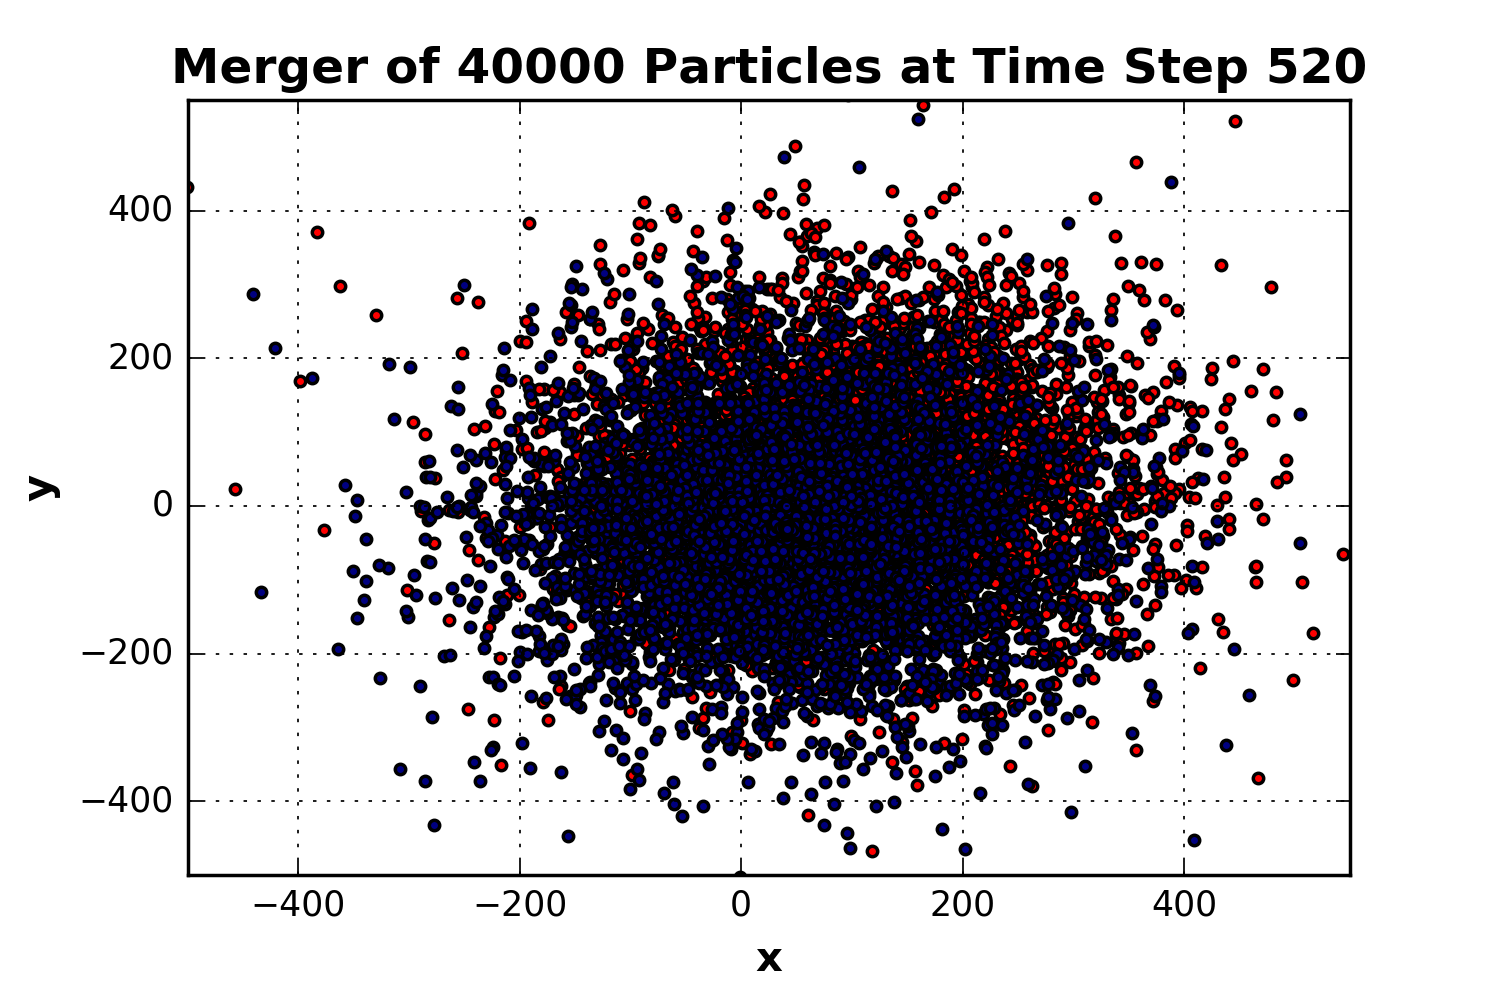
\includegraphics[width=\textwidth]{merger2_t520.png}\
            \caption[]%
            {{\small The two elliptical galaxies after the merger at a time step of $520$.}}
            \label{fig:merger2_t520}
        \end{subfigure}
        \caption[]
        {The plots above illustrate the second merger.}
        \label{fig:merger2}
    \end{figure}
    
  Figure~\ref{fig:merger2} shows the merging process of the two elliptical galaxies in the second model. Because the first set of galaxies did not spiral into one another, I decided to increase the initial x-shift between the two galaxies in hopes that the added distance would give the galaxies time to spiral. However, as can be seen in the figure above, this was not the case again. They just collided once more head-on with one another.
    
  
\begin{figure}[H]
\centering 
    \begin{subfigure}[b]{.475\textwidth}
        \centering
        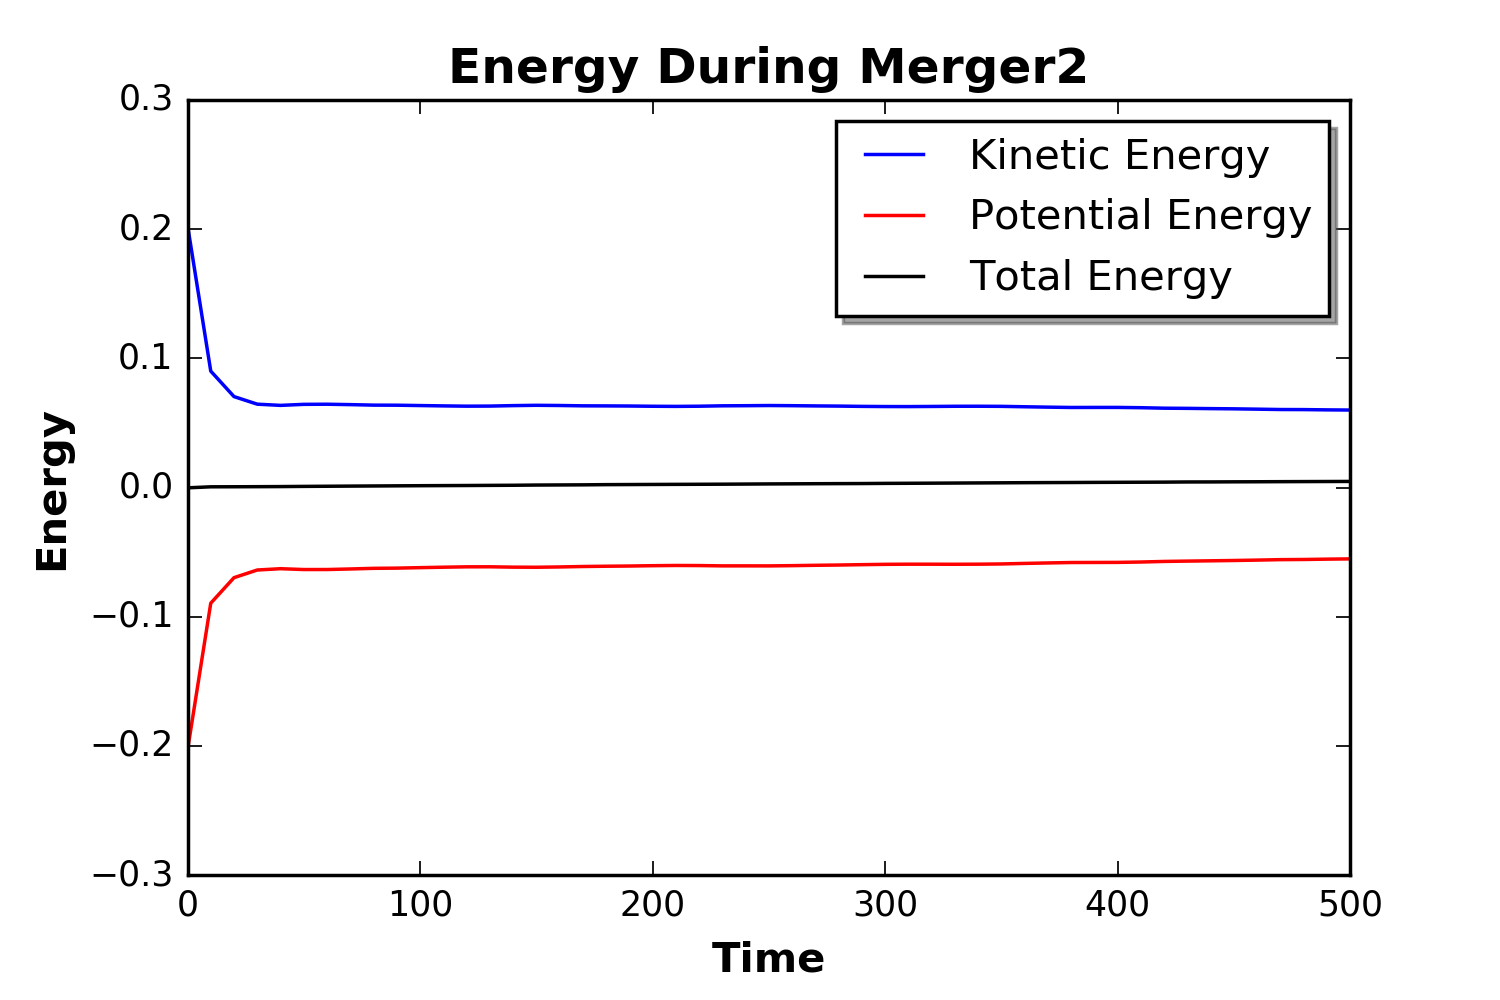
\includegraphics[width=\linewidth]{totenergy_merger2.png}
        \caption[]%
        {{Kinetic energy, potential energy, and total energy versus time.}}
    
        \label{fig:totalenergy_merger2}
    \end{subfigure} %'
    \hfill
    \begin{subfigure}[b]{.475\textwidth}
        \centering
        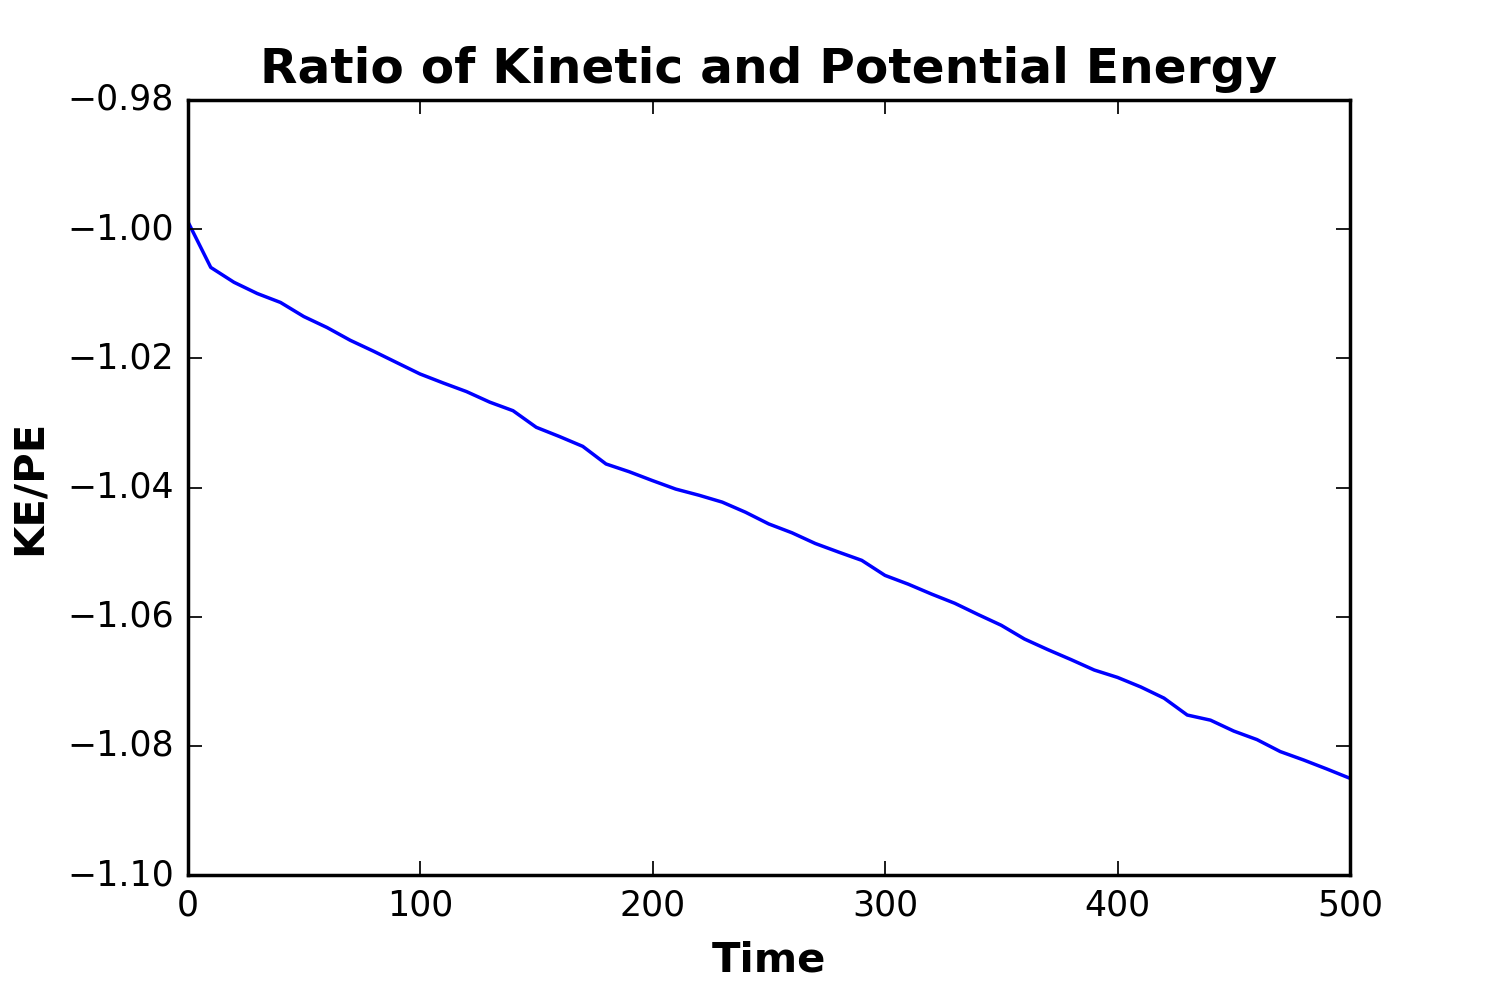
\includegraphics[width=\linewidth]{ratioenergy_merger2.png}
        \caption[]%
        {{The ratio between kinetic and potential energy versus time.}}
        \label{fig:ratiomerger2}
    \end{subfigure} %
    \caption[]
        {The plots above illustrate the energy change during the merger highlighted in Figure~\ref{fig:merger2}.} 
        \label{fig:energyofmerger2}
\end{figure}


Figure~\ref{fig:energyofmerger2} above illustrates the energy during the merger process seen in Figure~\ref{fig:merger2}. Unlike the first merger, there were no perturbations present in the kinetic and potential energies (if one compares Figures~\ref{fig:totalenergy} of merger 1 and \ref{fig:totalenergy_merger2} of merger 2. It all is pretty smooth. However, the main difference between these two plots is the ratio of kinetic energy to potential energy. This ratio for merger 2, as seen in Figure~\ref{fig:ratiomerger2}, is all negative and decreasing linearly; however, the ratio for merger 1, as seen in Figure~\ref{fig:ratiomerger1},  has a bump present at around a time step of $40$ before decreasing. This bump corresponds to when the mergers first began merging in Figure~\ref{fig:merger1_t040}.


\subsection*{Main Results}
\addcontentsline{toc}{subsection}{Main Results}

As seen in Table~\ref{tab:escapedparticles} in the Analytical Estimates section, quite a number of particles were lost in the initial formation of the elliptical galaxy ($\sim 344$ particles). The second merger configuration lost the most particles overall. It lost 
$10\%$ of its particles in comparison to the first merger that lost only about $2.4\%$ of its particles. This can likely be attributed to the fact that the second merger configuration was placed farther away from one another. Therefore, it had more time to lose more particles.

Furthermore, as seen in Figures~\ref{fig:density_initial}, \ref{fig:density_merger1}, and \ref{fig:density_merger2} exhibiting the density changes, all of the plots exhibit the same type of downward curve. The core of the system is the most dense, and density decreases as the radius increases. This makes sense because most of the particles are concentrated in the core.

In Figure~\ref{fig:density_initial}, there are some perturbations to the curve as the radius increases; however, these smooth out in Figures~\ref{fig:density_merger1} and \ref{fig:density_merger2}. Instead, the slight curve seen in Figure~\ref{fig:density_initial} at around a radius of $2$ increases in the following figures. Something interesting is that in Figure~\ref{fig:density_merger2}, there are two bumps present at a radius of $50$ and $110$. This could be an odd addition effect that occurred when summing over all of the radius bins and counting up the number of particles in each bin. 

However, the total angular momentum of each system is different. These differences can be seen in Figure~\ref{fig:angular_mmentum}. In Figure~\ref{fig:ang_merger1}, showing the first merger model, the total angular momentum is positive and big (in comparison to the second merger). There is a broad, square-like spike at a time step of around $40-50$, which indicates where the merger first happened in the first merger configuration. This corresponds to 
Figure~\ref{fig:merger1_t040}. The double spike seen between time steps $110$ and $160$ could be due to the fact that the two galaxies are separating from one another at this point after merging.

The angular momentum for the second merger is much lower overall. This can be seen in Figure~\ref{fig:ang_merger2}. Additionally, the plot is riddled with more frequent spikes. The moment of collision can probably be traced to the double, broad spike seen around time steps $110-190$, which seems to correspond closely to Figure~\ref{fig:merger2_t140}. 

The velocities of the two systems, seen in Figure~\ref{fig:velocity_of_mergers}, are also different. During merger 1, the velocities are mostly spiking up in the positive direction. An initial large spike is present in Figure~\ref{fig:velcoity_merger1} around a time step of $40-50$, which corresponds to the initial merging process of the first merger configuration seen in Figure~\ref{fig:merger1_t040}. However, the averaged velocities in the second merger configuration are spiking more numerously. The important part to note is in Figure~\ref{fig:velocity_merger2}, there is a sort of triple spike located around a time step of $140$. This likely corresponds to Figure~\ref{fig:merger2_t140}, which indicates that this is when the two galaxies collided.

\section*{Conclusion}
\addcontentsline{toc}{section}{Conclusion}

In conclusion, the merging of two elliptical galaxy configurations was explored. Both configurations were given the same initial velocity kicks while the x-direction offset was different. The first merger had an offset of $50$ in the x-direction, and the second merger had an offset of $150$ in the x-direction. Both were head-on collisions. The second merger ended up losing more particles, had a lower total angular momentum, lower velocities, and lower density, overall.

To gain a more conclusive insight into the merging process, I should have tested various merging scenarios with different time steps (dt) and changed the radius of the system.

\addcontentsline{toc}{section}{Bibliography}

\bibliographystyle{apj.bst}
\bibliography{bib.bib}
\end{document}


